\documentclass[9pt]{beamer}
\usetheme[progressbar=head,numbering=fraction]{metropolis}
\usepackage[utf8]{inputenc}
\usepackage[T1]{fontenc}
\usepackage{lmodern}

\usepackage{empheq}
\makeatletter
\colorlet{shadecolour}{blue!30}
\newcommand\Ashaded[1]{\let\bgroup{\romannumeral-`}\@Ashaded#1&&\ENDDNE}
\def\@Ashaded#1&#2&#3\ENDDNE{%
\ifnum0=`{}\fi \setbox \z@
\hbox{$\displaystyle#1{}\m@th$\kern\fboxsep \kern\fboxrule }%
\edef\@tempa {\kern \wd\z@ &\kern -\the\wd\z@ \fboxsep
\the\fboxsep }\@tempa \colorbox{shadecolour}{$#1#2 $}%
}
\colorlet{bgcolour}{yellow!20}
\colorlet{rulecolour}{blue!30}
\newcommand\Acolorboxed[1]{\let\bgroup{\romannumeral-`}\@Acolorboxed#1&&\ENDDNE}
\def\@Acolorboxed#1&#2&#3\ENDDNE{%
  \ifnum0=`{}\fi \setbox \z@
    \hbox{$\displaystyle#1{}\m@th$\kern\fboxsep \kern\fboxrule }%
    \edef\@tempa {\kern \wd\z@ &\kern -\the\wd\z@ \fboxsep
        \the\fboxsep\fboxrule \the\fboxrule }\@tempa \fcolorbox{rulecolour}{bgcolour}{$ #1#2 $}%
}
\makeatother

\usepackage{amsfonts,amsmath}
\allowdisplaybreaks

%\usepackage[export]{adjustbox}

% Tighter itemize
\expandafter\def\expandafter\normalsize\expandafter{%
    \normalsize%
    \setlength\abovedisplayskip{1pt}%
    \setlength\belowdisplayskip{1pt}%
    \setlength\abovedisplayshortskip{1pt}%
    \setlength\belowdisplayshortskip{1pt}%
}

\expandafter\def\expandafter\small\expandafter{%
    \small%
    \setlength\abovedisplayskip{1pt}%
    \setlength\belowdisplayskip{1pt}%
    \setlength\abovedisplayshortskip{1pt}%
    \setlength\belowdisplayshortskip{1pt}%
}

%\usepackage{beamerX}

%\setboolean{displaylogo}{false}

\AtBeginSection[]
{
\begin{frame}
        \frametitle{Outline}
        \tableofcontents[currentsection]
   \end{frame}
}
\AtBeginSubsection[]
{
\begin{frame}
        \frametitle{Outline}
        \tableofcontents[currentsection,currentsubsection]
   \end{frame}
}

\setbeamertemplate{frametitle continuation}[from second][]

\usepackage{graphicx}%

\newcommand{\parinc}[2]{\parbox[c]{#1}{\includegraphics[width=#1]{#2}}}
\newcommand{\parinch}[3]{\parbox[c][#2]{#1}{\includegraphics[width=#1]{#3}}}
\newcommand{\parincb}[3]{\parbox[c]{#1}{\includegraphics[width=#1,height=#2]{#3}}}

\usepackage{color}
\newcommand{\red}[1]{\textcolor{red}{#1}}

\usepackage{tikz}


\usepackage{scalerel,stackengine}
\stackMath
\newcommand\reallywidehat[1]{%
\savestack{\tmpbox}{\stretchto{%
  \scaleto{%
    \scalerel*[\widthof{\ensuremath{#1}}]{\kern-.6pt\bigwedge\kern-.6pt}%
    {\rule[-\textheight/2]{1ex}{\textheight}}%WIDTH-LIMITED BIG WEDGE
  }{\textheight}% 
}{0.5ex}}%
\stackon[1pt]{#1}{\tmpbox}%
}

\newcommand{\grad}{\nabla}
\newcommand{\ind}[1]{\mathbf{1}_{#1}}

\DeclareMathOperator{\limSup}{limsup}%
\DeclareMathOperator{\limInf}{liminf}%
\DeclareMathOperator*{\argmax}{argmax}%
\DeclareMathOperator*{\argmin}{argmin}%
\DeclareMathOperator*{\supp}{Supp}%
\DeclareMathOperator{\pen}{pen}
\DeclareMathOperator{\dom}{dom}
\DeclareMathOperator{\price}{price}
\DeclareMathOperator{\sign}{sign}
\DeclareMathOperator{\KL}{KL}
\DeclareMathOperator{\Proj}{Proj}
\DeclareMathOperator{\Span}{span}


\DeclareMathOperator*{\tr}{tr}
\DeclareMathOperator*{\ra}{rank}
\DeclareMathOperator*{\conv}{conv}
\DeclareMathOperator{\ve}{vec}
\DeclareMathOperator{\diag}{diag}

\newcommand{\R}{\mathbb{R}}
\newcommand{\Proba}{\mathbb{P}}
\newcommand{\Espe}{\mathbb{E}}
\newcommand{\Vari}{\mathbb{V}}
\newcommand{\Cova}{\mathbb{C}\text{ov}}
\newcommand{\Prob}[2][]{\Proba_{#1}\left(#2\right)}
\newcommand{\Esp}[2][]{\Espe_{#1}\left[#2\right]}
\newcommand{\Var}[2][]{\Vari_{#1}\left[#2\right]}
\newcommand{\Cov}[2][]{\Cova_{#1}\left[#2\right]}
\newcommand{\ud}{\textup{d}}
\newcommand{\charac}{\mathbf{1}}

\newcommand{\vecX}{\textbf{X}}
\newcommand{\transp}[1]{{#1}^t}

\usepackage{amsmath,amssymb,bbm,dsfont}
\usepackage{colortbl}
\usepackage{color}
\usepackage[T1]{fontenc}
\usepackage{psfrag}
\usepackage{graphicx}
\usepackage{multicol}
\usepackage{multirow}
\usepackage{tabularx}
\renewcommand{\d}{\delta}
\renewcommand{\a}{\alpha}
\newcommand{\e}{\varepsilon}
\newcommand{\F}{{\cal F}}
\newcommand{\s}{\sigma}
\newcommand{\Fd}{{\bf{F}}}
\def\P{\mathbbm P}

\newcommand{\bw}{\textbf{w}}
\newcommand{\eqsp}{\,}
\newcommand{\bx}{\textbf{x}}
\newcommand{\bX}{\textbf{X}}
\newcommand{\N}{\mathbbm{N}}
\newcommand{\un}{{\mathbbm{1}}}
\newcommand{\eqdef}{\stackrel{\Delta}{=}}
\newcommand{\E}{\mathbb E}
\newtheorem{defn}{Definition}
\newtheorem{thm}{Theorem}
\newtheorem{lem}{Lemma}
\newtheorem{cor}{Corollary}
\newtheorem{pro}{Proposition}
\newtheorem{prop}{Properties}

\definecolor{darkgreen}{rgb}{0.2,0.7,0.2}
\definecolor{nicegreen}{rgb}{0,0.667,0}
\definecolor{lightgreen}{rgb}{.667,1,.5}
\definecolor{lightblue}{rgb}{0,0.667,1}
\definecolor{orange}{rgb}{1,.333,0}
\definecolor{maroon}{rgb}{0.75,.25,0}
\definecolor{pink}{rgb}{1,0,1}
\definecolor{darkgray}{gray}{.3}
\newcommand{\white}[1]{\textcolor{white}{#1}}

\newcommand{\blue}[1]{\textcolor{blue}{#1}}
\newcommand{\green}[1]{\textcolor{green}{#1}}
\newcommand{\black}[1]{\textcolor{black}{#1}}
\newcommand{\nicegreen}[1]{\textcolor{nicegreen}{#1}}
\newcommand{\lightgreen}[1]{\textcolor{lightgreen}{#1}}
\newcommand{\lightblue}[1]{\textcolor{lightblue}{#1}}
\newcommand{\lightgray}[1]{\textcolor{lightgray}{#1}}
\newcommand{\pink}[1]{\textcolor{pink}{#1}}
\newcommand{\orange}[1]{\textcolor{orange}{#1}}
\newcommand{\maroon}[1]{\textcolor{maroon}{#1}}
\newcommand{\darkgray}[1]{\textcolor{darkgray}{#1}}
\newcommand{\yellow}[1]{\textcolor{yellow}{#1}}

\newcommand{\rank}[1]{\operatorname{rank}\p{#1}}
\newcommand{\nn}{\mathcal{N}}
\newcommand{\Norm}[1]{\left\lVert#1\right\rVert}

\newcommand{\law}{\mathcal{L}}
\newcommand{\EE}[2][]{\mathbb{E}_{#1}\left[#2\right]}
\newcommand{\simiid}{\,{\buildrel \text{iid} \over \sim\,}}
\newcommand{\p}[1]{\left(#1\right)}
\newcommand{\cX}{{\mathcal X}}%
\newcommand{\cY}{{\mathcal Y}}

\definecolor{violet}{cmyk}{0.79,0.88,0,0}
\definecolor{lightr}{RGB}{204,0,0}
% pour avoir le texte cach� en gris
% \beamertemplatetransparentcovereddynamic



%\pgfdeclareimage[width=1cm]{logoe}{LogoPetit}
%\pgfdeclareimage[width=1cm]{logoi}{LogoINRA-Couleur}

%\logo{\hbox {\tiny 4�mes Journ�es de Statistique Fonctionnelle}}
%\hskip 1.cm {\hbox to 1cm{
%      \hfil\pgfuseimage{logoe}}\hskip 1.cm\hbox{\pgfuseimage{logoi}}}}


%\beamertemplateshadingbackground{gray!0}{gray!50}
%\usepackage{beamerthemeshadow}

%\usetheme{Singapore}
%\setbeamercolor{background canvas}{bg=gray!10}
%\usepackage{beamerthemeclassic}

%\setbeamertemplate{headline}{}

%\setbeamertemplate{background canvas}[vertical shading][bottom=white!20,top=white!30]
%\usetheme{Rochester}
%  \usefonttheme[onlysmall]{structurebold}


\AtBeginSection[]
{
	\begin{frame}
	\frametitle{Outline}
	\tableofcontents[currentsection]
\end{frame}
}

\AtBeginSubsection[]
{
\begin{frame}
\frametitle{Outline}
\tableofcontents[currentsection,currentsubsection]
\end{frame}
}
\title[Introduction to machine learning]{MSc Big Data for Business - {\em MAP 534} \\
Introduction to machine learning\\}

\newcommand{\inr}[1]{\langle #1 \rangle}
\newcommand{\norm}[1]{\|#1\|}

\author{}
\date{}

\begin{document}

\author[S. Le Corff]{\textcolor{violet}{Supervised classification}\\ {\em {\small \textcolor{violet}{Linear/Quadratic discriminant analysis (LDA/QDA) \& Support Vector Machines (SVM)}}}}


\begin{frame}
  \maketitle 
\end{frame}


\begin{frame}[allowframebreaks]
\frametitle{Machine Learning}
\begin{center}
	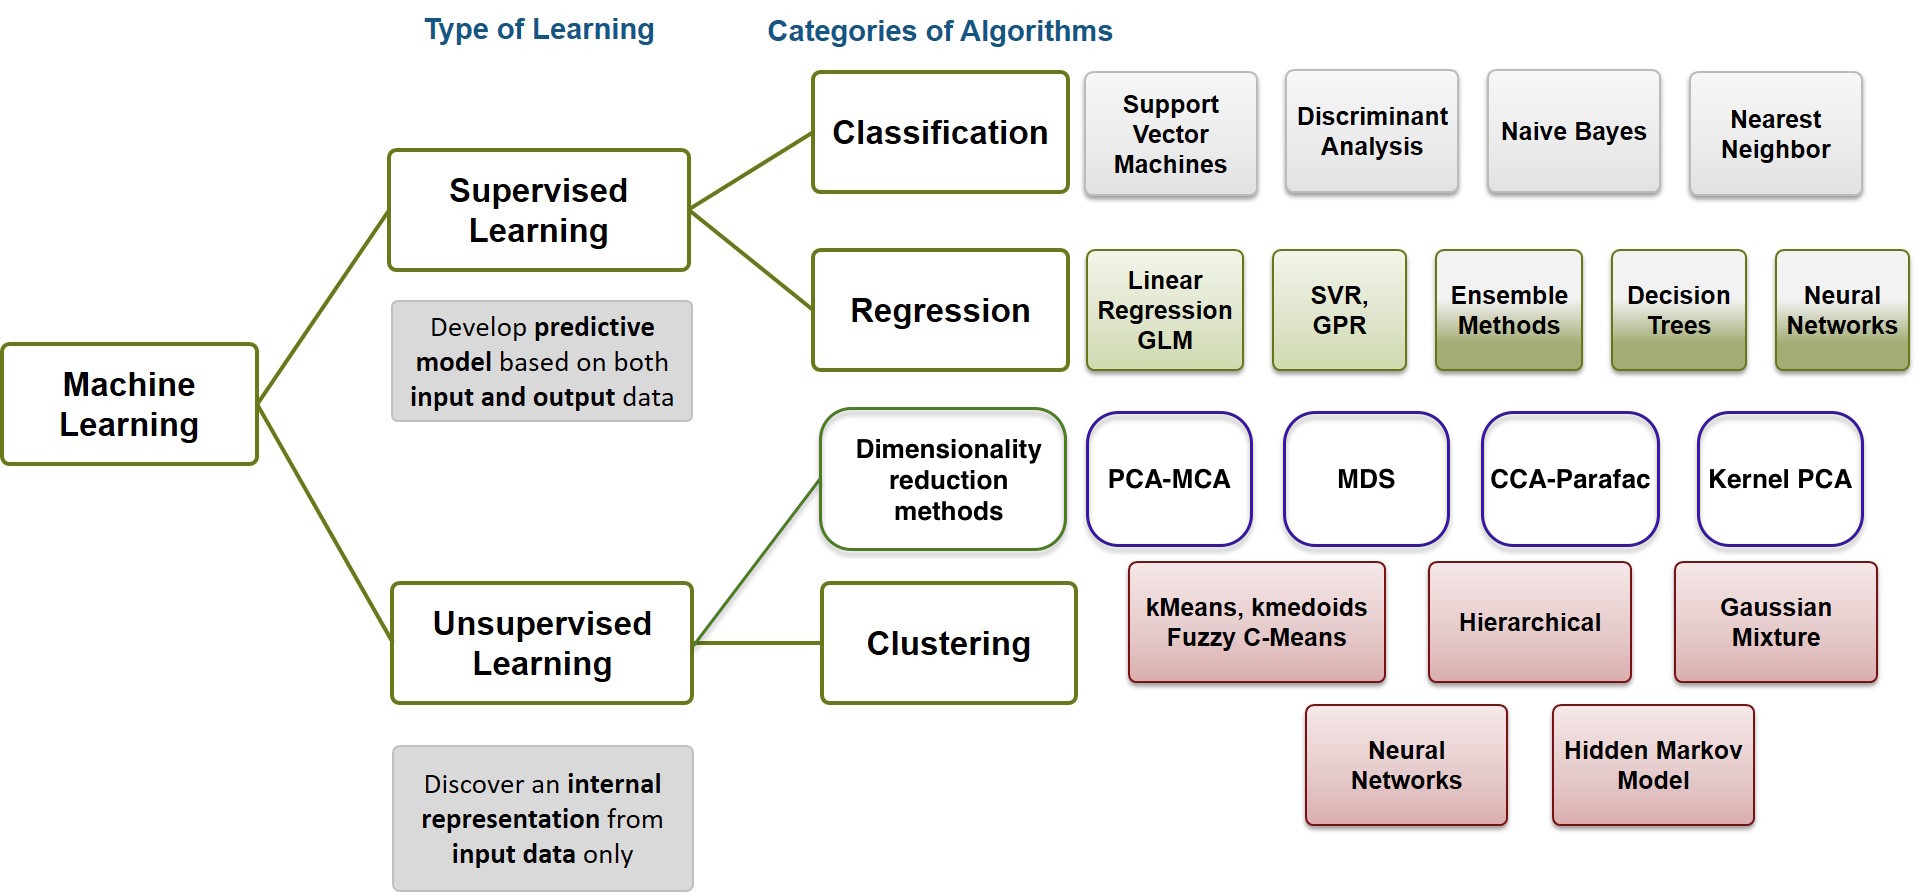
\includegraphics[width=\textwidth]{Learning+Types.jpg}
\end{center}
\end{frame}


\section{Introduction to supervised learning}

\begin{frame} \frametitle{Supervised  Learning}
\textcolor{violet}{{\bf Supervised Learning Framework}}

$\rightharpoondown$ \alert{Input} measurement $\textbf{X}  \in \mathcal{X}$ (often $\mathcal{X} \subset \R^d$), \alert{output} measurement $Y \in \mathcal{Y}$.

$\rightharpoondown$  The joint distribution of $(\textbf{X},Y)$ is  \alert{unknown}.

$\rightharpoondown$  $Y \in \{-1,1\}$ (classification) or $Y \in \mathbb{R}^m$ (regression).


$\rightharpoondown$ A \alert{predictor} is a measurable function in $\mathcal{F} = \{ f:\mathcal{X} \to \mathcal{Y}\}$.

\vspace{.5cm}

\textcolor{violet}{{\bf Training data}}

$\rightharpoondown$ $\mathcal{D}_n=\{(\textbf{X}_1, Y_1),\ldots,(\textbf{X}_n, Y_n)\}$ i.i.d. with the same distribution as $(\textbf{X},Y)$.




\vspace{.5cm}

\textcolor{violet}{{\bf Goal}}

$\rightharpoondown$  Construct a \alert{good} predictor $\widehat{f}_n$ from the training data.

$\rightharpoondown$  Need to specify the meaning of good.

\end{frame}

\begin{frame}
\frametitle{Loss and Probabilistic Framework}
\textcolor{violet}{{\bf Loss function}}

$\rightharpoondown$ $\ell(Y,f(\textbf{X}))$ measures the goodness of the prediction of $Y$ by $f(\textbf{X})$.

$\rightharpoondown$ \alert{Prediction} loss: $\ell(Y,f(\textbf{X}))=\mathbf{1}_{Y\neq f(\textbf{X})}$.

$\rightharpoondown$  \alert{Quadratic} loss: $\ell(Y,\textbf{X})=\|Y-f(\textbf{X})\|^2$.

\vspace{.5cm}

\textcolor{violet}{{\bf Risk function}}

$\rightharpoondown$ Risk measured as the average loss:
	\[
	\alert{\mathcal{R}(f)=\Esp{\ell(Y,f(\textbf{X}))}}\,.
	\]

$\rightharpoondown$ \alert{Prediction} loss: $\Esp{\ell(Y,f(\textbf{X}))}=\Prob{Y\neq f(\textbf{X})}$.

$\rightharpoondown$ \alert{Quadratic} loss: $\Esp {\ell(Y,f(\textbf{X}))}=\Esp{\|Y-f(\textbf{X})\|^2}$.

\vspace{.3cm}

$\rightharpoondown$ \textcolor{lightr}{\textbf{Beware:}}  As $\widehat{f}_n$ depends on $\mathcal{D}_n$, $\mathcal{R}(\widehat{f}_n)$ is a random variable!

\end{frame}


\begin{frame}
\frametitle{A robot that learns}
\textcolor{violet}{A robot endowed with a set of sensors} and an online learning algorithm.
\begin{center}
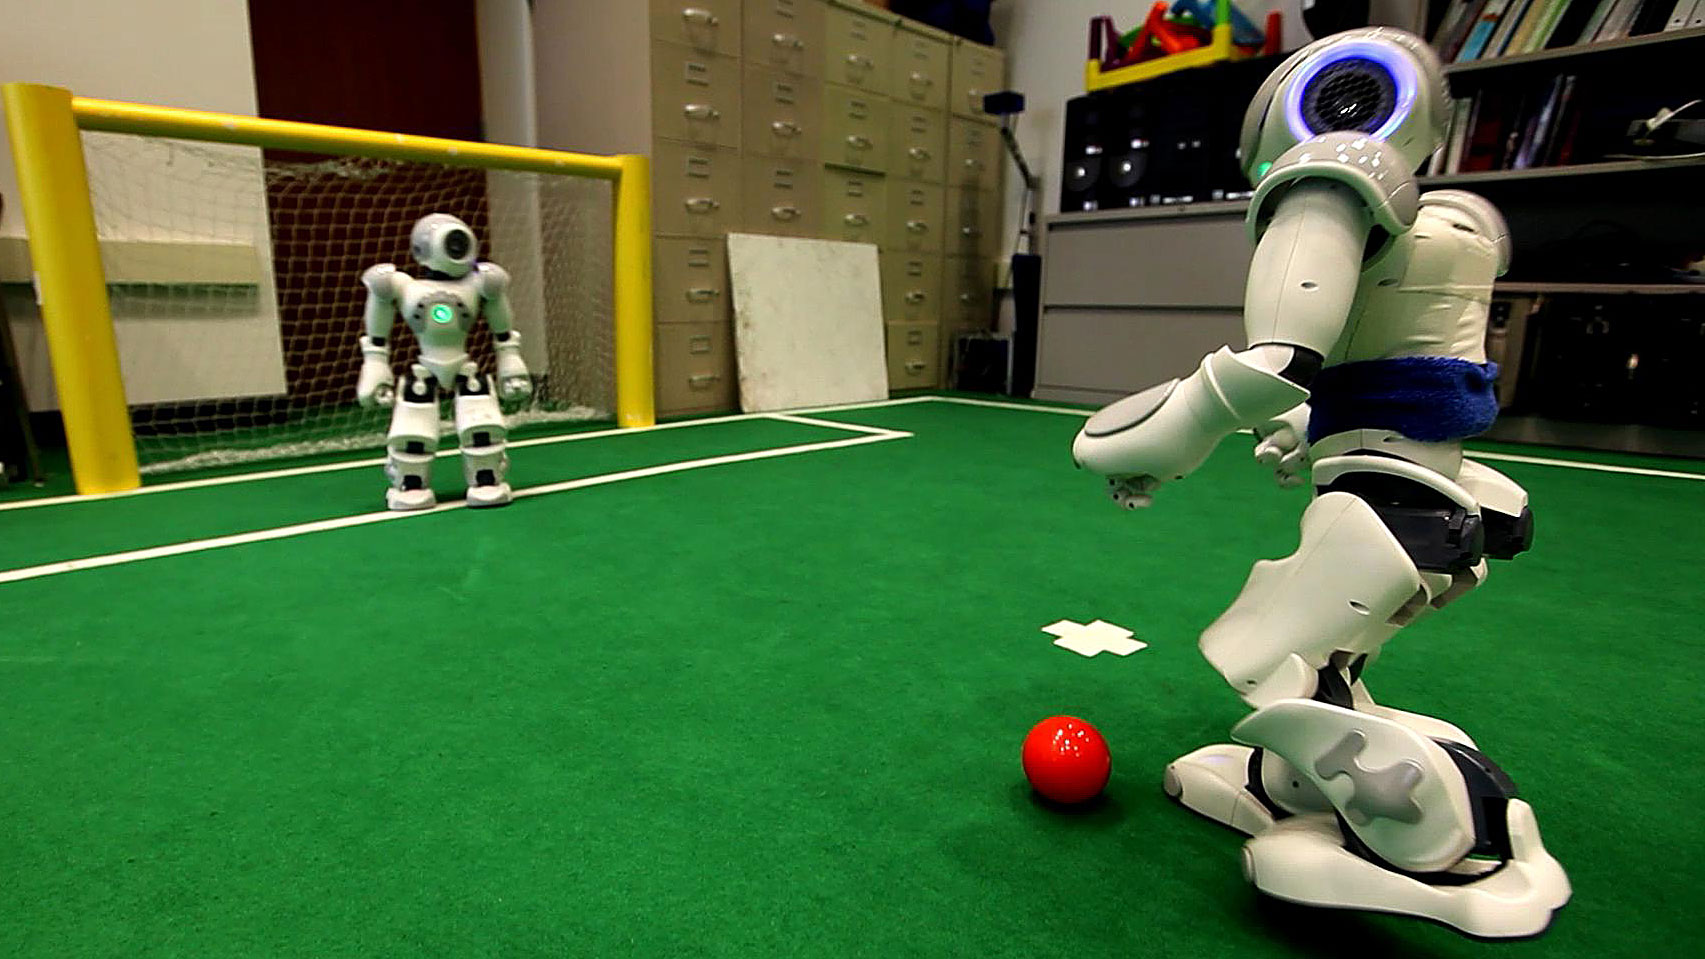
\includegraphics[width=5cm]{soccer-playing-robots}
\end{center}

$\rightharpoondown$   \alert{Task}: play football.
 
$\rightharpoondown$  \alert{Performance}: score.

$\rightharpoondown$  \alert{Experience}: current environment and outcome, past games...

\end{frame}

\begin{frame}
\frametitle{Object recognition in an image}
\centerline{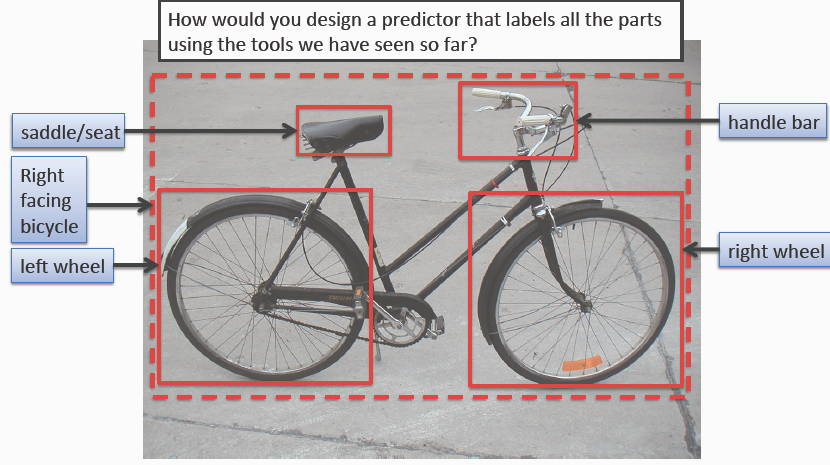
\includegraphics[width=.8\textwidth]{object-detection}}
\vspace*{.5cm}

$\rightharpoondown$   \alert{Task}: say if an object is present or not in the image.

$\rightharpoondown$  \alert{Performance}:  number of errors.

$\rightharpoondown$  \alert{Experience}: set of previously seen labeled image.

\end{frame}


\begin{frame}
	\frametitle{Number}
	\centerline{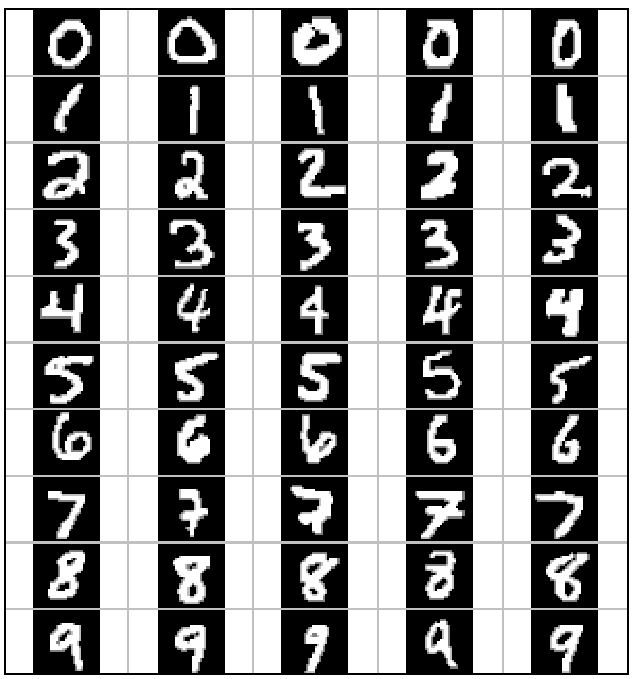
\includegraphics[width=.4\textwidth]{mnist}}
	\vspace*{.3cm}

$\rightharpoondown$   \alert{Task}: Read a ZIP code from an envelop.

$\rightharpoondown$  \alert{Performance}:  give a number from an image.

$\rightharpoondown$  \textcolor{violet}{Prediction problem} with $\vecX$:  image and $Y$: corresponding number.

\end{frame}

\begin{frame}
	\frametitle{Applications in biology}
	\centerline{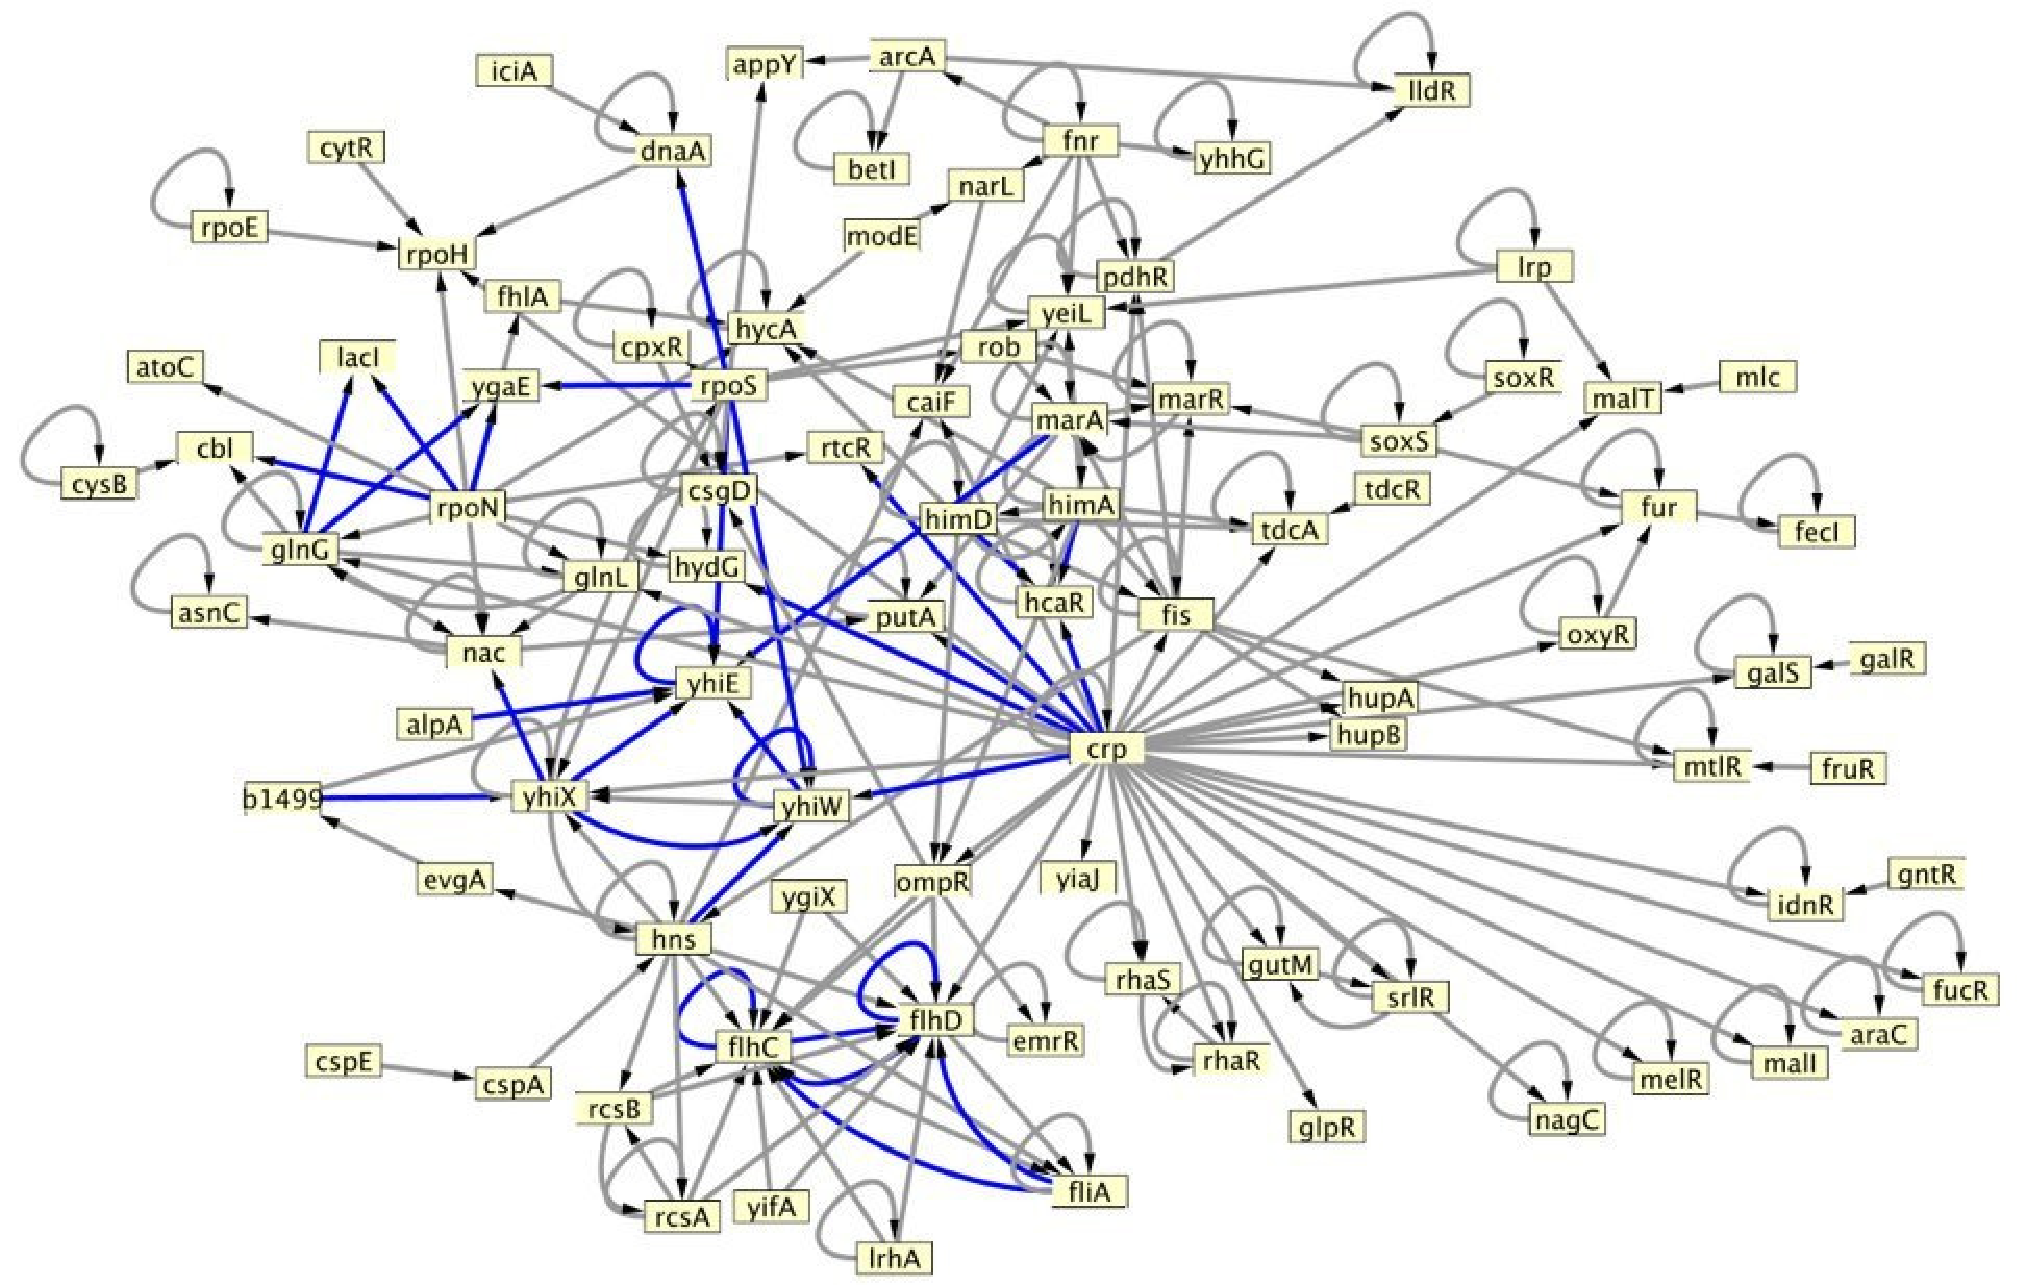
\includegraphics[width=.6\textwidth]{bio}}

$\rightharpoondown$   \alert{Task}: protein interaction network prediction.

$\rightharpoondown$  \alert{Goal}: predict (unknown) interactions between proteins.

$\rightharpoondown$  \textcolor{violet}{Prediction problem} with $\vecX$: pair of proteins and $Y$: existence or no of interaction.

%Numerous similar questions in bio(informatics), genomic, etc.

\end{frame}

\begin{frame}
	\frametitle{Detection}
	\centerline{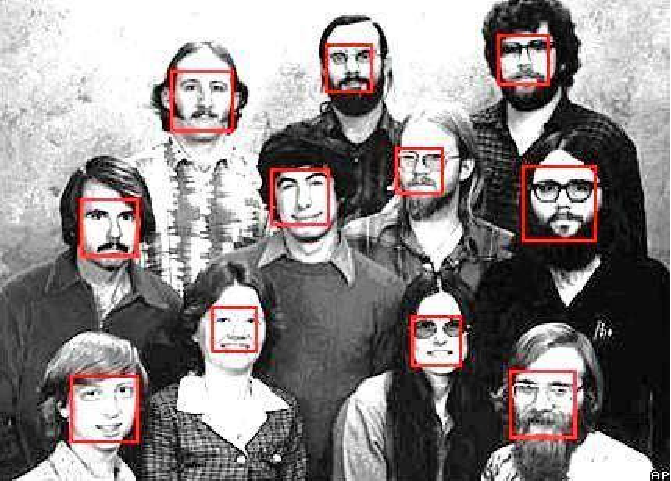
\includegraphics[width=6cm]{faces}}

$\rightharpoondown$  \alert{Goal}: detect the position of faces in an image.


$\rightharpoondown$  $\vecX$: mask  in the image and $Y$: presence or no of a face...

%Lots of answer in a single image. Post processing required...

\end{frame}

\begin{frame}{Classification}

\textcolor{violet}{{\bf Setting}}

$\rightharpoondown$ Historical data  about \alert{individuals $i=1, \ldots, n$}.

$\rightharpoondown$ \textbf{Features} vector $\bX_i \in \R^d$ for each individual $i$.

$\rightharpoondown$ For each $i$, the individual \alert{belongs to a group} ($Y_i = 1$) or not ($Y_i = -1$).

$\rightharpoondown$ $Y_i \in \{ -1, 1 \}$ is  the \textbf{label} of $i$.


\vspace{.6cm}

\textcolor{violet}{{\bf Aim}}

$\rightharpoondown$ Given a new $\bX$ (with no corresponding label), \alert{predict a label in $\{ -1, 1 \}$}.

$\rightharpoondown$ Use data $\mathcal{D}_n = \{ (\bx_1, y_1), \ldots, (\bx_n, y_n) \}$ \alert{to construct a  \textbf{classifier}}.


\end{frame}


\begin{frame}[t]
\frametitle{Classification}

\textcolor{violet}{{\bf Geometrically}}
\begin{center}
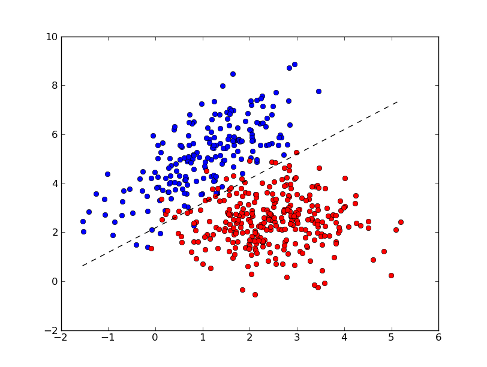
\includegraphics[width=0.7\textwidth]{./lda_binary.png}  
\end{center}
Learn a \alert{boundary to separate two ``groups''} of points.
\end{frame}


\begin{frame}[t]
\frametitle{Classification}

...many ways to separate points!

\begin{center}
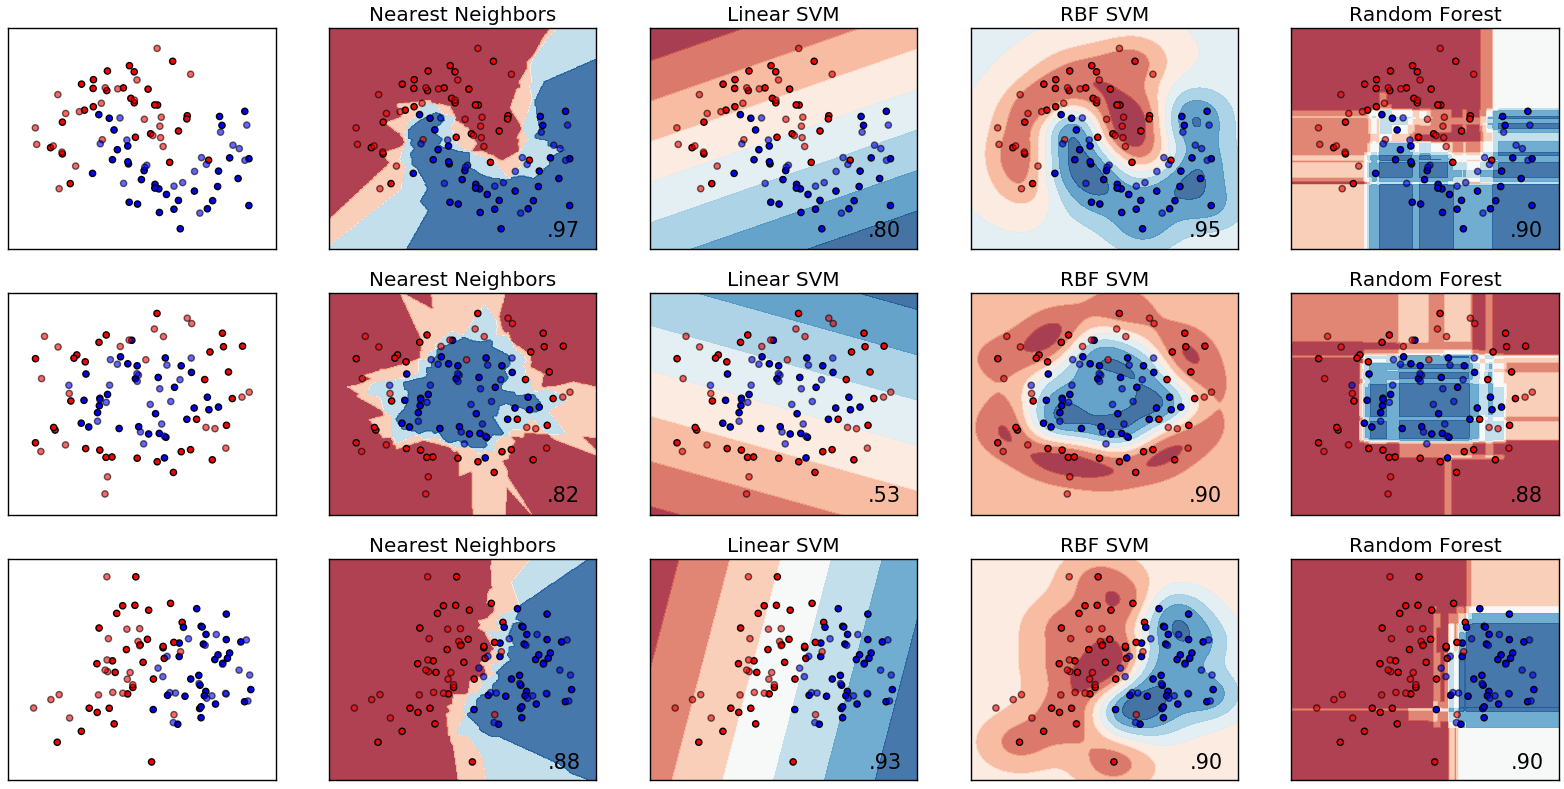
\includegraphics[width=1\textwidth]{./classifier_comparison.png}
\end{center}
\end{frame}

\begin{frame}[allowframebreaks]
\frametitle{Supervised learning methods}


\textcolor{violet}{Support Vector Machine}

\vspace{.2cm}

\textcolor{violet}{Linear Discriminant Analysis}

\vspace{.2cm}

Logistic Regression

\vspace{.2cm}

Trees/ Random Forests

\vspace{.2cm}

\textcolor{violet}{Kernel methods}

\vspace{.2cm}

Neural Networks

\vspace{.2cm}

Many more...


\end{frame}





\section{Bayes and Plug-in classifiers}


\begin{frame}
\frametitle{Best Solution}

\alert{The best solution} $f^*$ (which is independent of $\mathcal{D}_n$) is 

\begin{align*}
\Acolorboxed{f^* &= \arg\min_{f \in \mathcal{F}} R(f) = \arg\min_{f \in \mathcal{F}}
	\Esp{\ell(Y,f(\textbf{X}))}\eqsp.}
\end{align*}

\vspace{.3cm}

\textcolor{violet}{{\bf Bayes Predictor (explicit solution)}}

$\rightharpoondown$ \alert{Binary classification} with $0-1$ loss: 
			\begin{align*}
			f^*(\textbf{X}) = \begin{cases}
			+1 & \text{if  \, $\Prob{Y=1\middle|\textbf{X}} \geqslant \Prob{Y=-1\middle| \textbf{X}}$}\\
			& \text{ $\Leftrightarrow \Prob{Y=1\middle|\textbf{X}} \geqslant 1/2$}\,,\\
			-1 & \text{otherwise}\,.
			\end{cases}
			\end{align*}

$\rightharpoondown$ \alert{Regression} with the quadratic loss
			\begin{align*}
			f^*(\textbf{X}) = \Esp{Y\middle|\textbf{X}}\,.
			\end{align*}


The explicit solution requires to \alert{know $\Esp{Y|\textbf{X}}$}...

\end{frame}


\begin{frame}
\frametitle{Plugin Classifier}

$\rightharpoondown$ In many cases, \alert{the conditional law of $Y$ given $\bX$ is not known}... or relies on parameters \alert{to be estimated}.

$\rightharpoondown$ An \alert{empirical surrogate of the Bayes classifier} is obtained from a possibly nonparametric estimator  $\widehat\eta_n(\bX)$ of 

\begin{align*}
\Acolorboxed{\eta(\bx) &= \mathbb{P}(Y=1|\bX)}
\end{align*}

\vspace{.2cm}

\textcolor{lightr}{using the training dataset}.

$\rightharpoondown$  This surrogate is then \alert{plugged into the Bayes classifier}.


\vspace{.5cm}

\textcolor{violet}{{\bf Plugin Bayes Classifier}}

\vspace{.2cm}

$\rightharpoondown$  \alert{Binary classification} with $0-1$ loss: 
 \begin{align*}
 \widehat{f}_n(\vecX) = \begin{cases}
 +1 & \text{if  \, $\widehat\eta_n(\bX) \geqslant 1/2$}\,,\\
-1 & \text{otherwise}\,.
     \end{cases}
   \end{align*}


\end{frame}


\begin{frame}
	\frametitle{Plugin Classifier}

\textcolor{violet}{{\bf Input}}: a data set $\mathcal{D}_n$.

Learn \alert{the ditribution of $Y$ given $\bX$} (using the data set) and plug this estimate in the Bayes classifier. 
		
\vspace{0.3cm}

\textcolor{violet}{{\bf Output}}: a classifier $\widehat{f}_n: \mathbb{R}^d \to \{-1,1\}$

			\begin{align*}
			\widehat{f}_n(\vecX) = \begin{cases}
			+1 & \text{if $\widehat{\eta}_n(\vecX)\geqslant 1/2$}\,,\\
			-1 & \text{otherwise}\,. 
			\end{cases}
			\end{align*}

\vspace{.4cm}

$\rightharpoondown$ Can we certify that the \alert{plug-in classifier is good} ?

\end{frame}




\begin{frame}
\frametitle{Classification Risk Analysis}

The missclassification error satisfies (\alert{see exercices}):

\vspace{.3cm}

\begin{align*}
\Acolorboxed{&0 \leqslant \mathbb{P}(\widehat{f}_n(\bX) \neq Y) - L^{\star} \leqslant 2\mathbb{E}\left[\left|\eta(\vecX) - \hat{\eta}_n(\vecX)\right|^2\right]^{1/2} \eqsp,}
\end{align*}

\vspace{.2cm}

where
$$
L^{\star} = \mathbb{P}(f^{\star}(\bX) \neq Y)
$$

\vspace{.2cm}

and  $\widehat{\eta}_n(\bx)$ is \alert{an empirical estimate based on the training dataset} of

\vspace{.2cm}

$$
\eta(\bx) = \mathbb{P}(Y=1|\bX = \bx)\,.
$$

		

\end{frame}



\begin{frame}
  \frametitle{How to estimate the conditional law of $Y$?}


\textcolor{violet}{{\bf Fully parametric modeling.}}
    
     Estimate the law of $(\vecX,Y)$
      and use the \textbf{Bayes formula} to deduce an estimate of
      the conditional law of $Y$: \emph{LDA/QDA, Naive Bayes...}

\vspace{.3cm}

\textcolor{violet}{{\bf Parametric conditional modeling.}}
    
     Estimate the conditional law of
      $Y$ by a \textbf{parametric} law: \emph{linear regression, logistic regression, Feed Forward Neural Networks...}

\vspace{.3cm}

\textcolor{violet}{{\bf Nonparametric conditional modeling.}}
    
     Estimate the conditional  law of
      $Y$ by a \textbf{non parametric} estimate: \emph{kernel
        methods, nearest neighbors...}

 
\end{frame}


% \begin{frame}
%   \frametitle{Risk Analysis (Proof)}
%   \begin{itemize}\small
%     \item Let us denote $p_1(\vecX) = \Prob{Y=1|\vecX}$
%   \item Step 1: Let $\tilde{f}(\vecX)= \sign(2 \tilde{p}_1(\vecX)-1)$
%     \begin{align*}
%       \Esp{\ell^{0/1}(Y,\tilde{f}(\vecX))} 
%       &= \Esp[\vecX]{p_{1}(\vecX)
%         \mathbf{1}_{\tilde{f}(\vecX)=-1} + (1- p_{1}(\vecX))
%         \mathbf{1}_{\tilde{f}(\vecX)=1}}\\
%       & = \Esp[\vecX]{(1-p_{1}(\vecX)) + (2 p_1(\vecX)-1) \mathbf{1}_{\tilde{f}(\vecX)=-1}}
%     \end{align*}
% \item Step 2:
%   \begin{align*}
% &\mspace{-45mu}    \Esp{\ell^{0/1}(Y,\tilde{f}(\vecX))} -
%     \Esp{\ell^{0/1}(Y,\tilde{f}^{\star}(\vecX))}\\
% & = \Esp[\vecX]{(2 p_1(\vecX)-1)
%   (\mathbf{1}_{\tilde{f}(\vecX)=-1}-\mathbf{1}_{f^{\star}(\vecX)=-1})}\\
% \intertext{using the definition of $f^{\star}= \sign(2p(\vecX-1)$}
% & = \Esp[\vecX]{|2p_1(\vecX)-1|
%   \mathbf{1}_{f^{\star}(\vecX)\neq\tilde{f}(\vecX)}}
% \intertext{and using the fact that
%   $f^{\star}(\vecX)\neq\tilde{f}(\vecX)$ implies that
%   $\widehat{p}(\vecX)$ and $p(\vecX)$ are not on the same
%   side with respect to $1/2$}
% & \leq
%   2\Esp[\vecX]{|p_1(\vecX)-\widehat{p}_{1}(\vecX)|} ) =
%   \Esp[\vecX]{\|p(\vecX)-\widehat{p}(\vecX)\|_1}\\
% \intertext{using $\|P-Q\|_1 \leq \sqrt{2\text{KL}(P,Q)}$ and Jensen}
% & \leq
%   \Esp[\vecX]{\sqrt{2\text{KL}(p(\vecX),\widehat{p}(\vecX))}}
% \leq \left(
%   \Esp[\vecX]{2\text{KL}(p(\vecX),\widehat{p}(\vecX))}
%   \right)^{1/2}
%   \end{align*}
%   \end{itemize}
% \end{frame}

%\section{Parametric models}

%\subsection{Linear/quadratic  discriminant analysis}

\begin{frame}
  \frametitle{Fully Generative Modeling}


If the law of $(\vecX,Y)$ \textcolor{lightr}{{\bf is known}}  everything can  be easy!

\textcolor{violet}{{\bf Bayes formula}}

 With a slight abuse of notation, if \alert{the law of $\vecX$ has a density $g$} with respect to a reference measure,
\begin{align*}
\Acolorboxed{&\Prob{Y= k| \vecX}   = \frac{g_k(\vecX)\Prob{Y=k}}{g(\vecX)}\eqsp,}
\end{align*}

where $g_k$ is the density of the distribution of $\bX$ given $\{Y = k\}$.

\vspace{.2cm}

\textcolor{violet}{{\bf Generative Modeling}}


\alert{Propose a model} for $(\vecX,Y)$.

\alert{Plug the conditional law of Y given $\bX$} in the Bayes \emph{classifier}.

\vspace{.3cm}

\textcolor{violet}{{\bf Remark:}} require to model the joint law of $(\vecX,Y)$ rather than only
  the conditional law of $Y$.

Great flexibility in the model design but may lead to complex computation.

\end{frame}

%\begin{frame}
%\frametitle{Fully Generative Modeling}
%
%\textcolor{lightr}{{\bf Simplest setting}} in classification!
%
%
%\textcolor{violet}{{\bf Bayes formula}}
%
%  \begin{align*}
% \Prob{Y = k|\vecX}= \frac{\Prob{\vecX|Y=k}\Prob{Y=k}}{\Prob{\vecX}}\,.
%  \end{align*}
%
%
%
%Binary Bayes classifier (the best solution).
%  \begin{align*}
%    f^*(\vecX) = \begin{cases}
%+1 & \text{\small if $\Prob{Y=1|\vecX} \geq \Prob{Y=-1|\vecX}$}\,,\\
%-1 & \text{otherwise}\,. 
%    \end{cases}
%  \end{align*}
%
%\textcolor{violet}{{\bf Heuristic}}: estimate those quantities and plug the estimations.
%Choosing  different models/estimators for $\Prob{\vecX\middle|Y}$ leads to  different classifiers.
%
%\textbf{Remark:} no need to renormalize by $\Prob{\vecX}$ to take the decision!
%
%\end{frame}

\section{Naive Bayes}

\begin{frame}{Naive Bayes}

\textcolor{violet}{{\bf Naive Bayes}}

Classical algorithm using a crude modeling for $\Prob{\vecX\middle| Y}$:

$\rightharpoondown$ \alert{Feature  independence} assumption:
\begin{align*}
\Prob{\vecX\middle|Y}=\prod_{i=1}^d \Prob{X^{(i)}\middle|Y}\,.
\end{align*}

$\rightharpoondown$ \alert{Simple featurewise model}: binomial if binary, multinomial if finite and Gaussian if continuous. 

\vspace{.2cm}

If all features are continuous, the law of $\bX$ given $Y$ is Gaussian with a \alert{{\bf diagonal covariance matrix}}!

\vspace{.2cm}

Very simple learning even in \textcolor{lightr}{very high dimension!}

\end{frame}

\begin{frame}{Gaussian Naive Bayes}
$\rightharpoondown$ \alert{Feature  independence} assumption:
\begin{align*}
\Prob{\vecX\middle|Y}=\prod_{j=1}^d \Prob{X^{(j)}\middle|Y}\,.
\end{align*}
For $k\in\{-1,1\}$, \textcolor{violet}{$\Prob{Y=k} = \pi_k$} and the \textcolor{violet}{conditional density of $X^{(j)}$ given $\{Y = k\}$} is 

\begin{align*}
\Acolorboxed{& g_k(\bx^{(j)}) = (2\pi\sigma^2_{j,k})^{-1/2}\mathrm{exp}\left\{-(\bx^{(j)}-\mu_{j,k})^2/(2\sigma^2_{j,k})\right\}\eqsp.}
\end{align*}

\vspace{.2cm}

The conditional distribution of $\bX$ given $\{Y = k\}$ is then

\begin{align*}
\Acolorboxed{& g_k(\bx) = (\mathrm{det}(2\pi \Sigma_k))^{-1/2}\mathrm{exp}\left\{-(\bx-\mu_{k})^T\Sigma_k^{-1}(\bx-\mu_{k})/2\right\}\eqsp,}
\end{align*}

\vspace{.2cm}

where \textcolor{violet}{$\Sigma_k = \mathrm{diag}(\sigma_{1,k}^2,\ldots,\sigma_{d,k}^2)$} and \textcolor{violet}{$\mu_k = (\mu_{1,k},\ldots,\mu_{d,k})^T$}.

\end{frame}

\begin{frame}{Gaussian Naive Bayes}
In a two-classes problem, the optimal classifier is (\alert{see linear discriminant analysis below}):

\begin{align*}
\Acolorboxed{&f^*:\bX\mapsto 2\mathds{1}\{\Prob{Y= 1| \vecX}>\Prob{Y= -1| \vecX}\}-1\eqsp.}
\end{align*}

\vspace{.2cm}

$\rightharpoondown$ When the parameters are unknown, they may be replaced by their \alert{maximum likelihood estimates}.

This yields, for $k\in\{-1,1\}$,  
\begin{align*}
\textcolor{violet}{{\bf \widehat \pi_k^n}} &= \frac{1}{n}\sum_{i=1}^n\mathds{1}_{Y_i=k}\,,\\
\textcolor{violet}{{\bf \widehat \mu_k^n}} &= \frac{1}{\sum_{i=1}^n\mathds{1}_{Y_i=k}}\sum_{i=1}^n\mathds{1}_{Y_i=k}\,X_i\,,\\
\textcolor{violet}{\widehat\Sigma_k^n} &= \mathrm{diag}\left(\frac{1}{n}\sum_{i=1}^n \left(X_i - \widehat \mu_{k}^n\right)\left(X_i - \widehat \mu_{k}^n\right)^T\mathds{1}_{Y_i=k}\right)\,.
\end{align*}

\end{frame}

\begin{frame}{Gaussian Naive Bayes}
\begin{center}
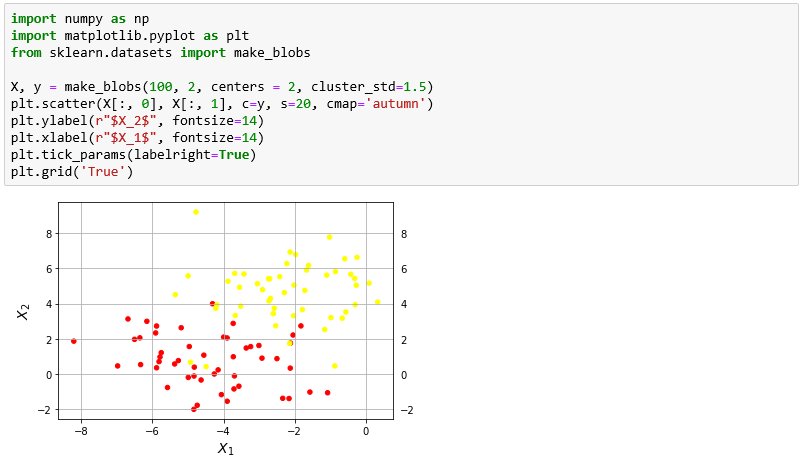
\includegraphics[width=0.9\linewidth]{./naivebayes_data}
\end{center}
\end{frame}

\begin{frame}{Gaussian Naive Bayes}
\begin{center}
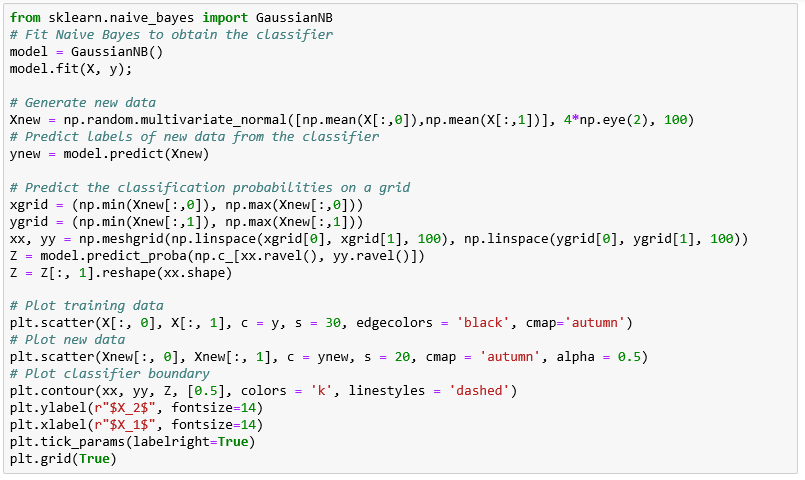
\includegraphics[width=\linewidth]{./naivebayes_classif1}
\end{center}
\end{frame}

\begin{frame}{Gaussian Naive Bayes}
\begin{center}
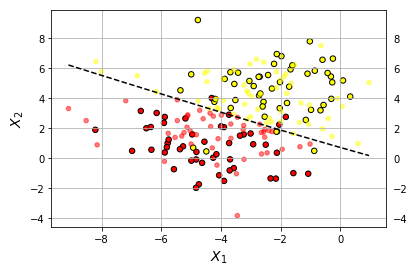
\includegraphics[width=0.8\linewidth]{./naivebayes_classif2}
\end{center}
\end{frame}

\begin{frame}{Gaussian Naive Bayes }
\begin{center}
\hspace*{-.05\textwidth}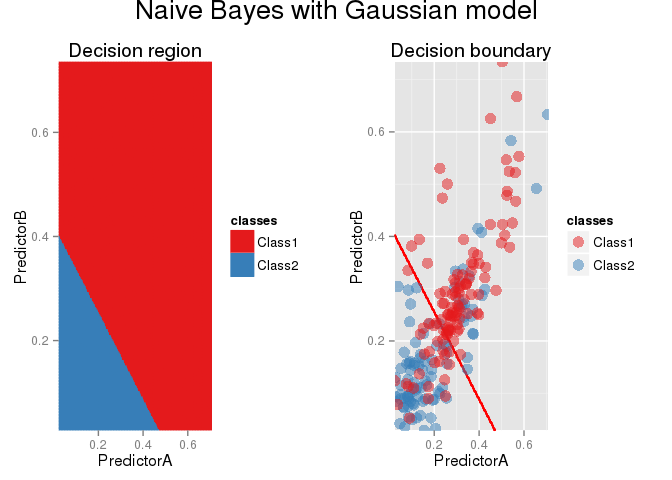
\includegraphics[height=.65\textheight]{Classical_Naive_Bayes-1}
\end{center}
\end{frame}

\begin{frame}
\frametitle{Kernel density estimate based Naive Bayes }
\begin{center}
\hspace*{-.05\textwidth}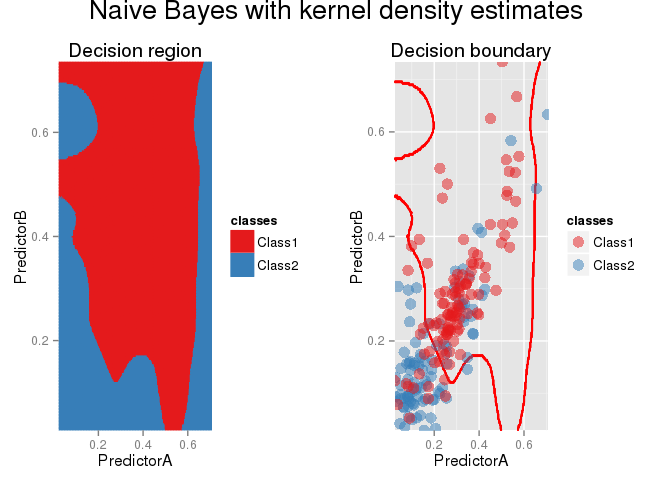
\includegraphics[height=.65\textheight]{Naive_Bayes_with_kernel_density_estimation-1}
\end{center}
\end{frame}

\section{Discriminant analysis (linear and quadratic)}


\begin{frame}[allowframebreaks]
\frametitle{Discriminant Analysis}
\vspace*{-.4cm}

\textcolor{violet}{{\bf Discriminant Analysis (Gaussian model)}}

The \alert{conditional densities are modeled as multivariate normal}. For all class $k$, conditionnally on $\{Y=k\}$,
\begin{align*}
\vecX\sim \mathcal{N}(\mu_k, \Sigma_k)\,.
\end{align*}

\textcolor{lightr}{Discriminant functions}:

$$
g_k(\vecX) = \ln (\mathbb{P}\{\vecX|Y=k\}) + \ln(\Prob{Y=k})
\eqsp.
$$

In a two-classes problem, the optimal classifier is (\alert{see exercises}):

\begin{align*}
\Acolorboxed{&
f^*:x\mapsto 2\mathds{1}\{g_1(x)>g_{-1}(x)\}-1\eqsp.}
\end{align*}


\vspace{.5cm}


\textcolor{violet}{QDA (differents $\Sigma_k$ in each class)}  and \textcolor{violet}{LDA ($\Sigma_k=\Sigma$ for all $k$)} 


\textcolor{violet}{lightr}: this model can be false but the methodology remains valid!

\framebreak

\textcolor{violet}{{\bf Estimation}} 


In practice, $\mu_k$, $\Sigma_k$ and $\pi_k:=\Prob{Y=k}$ have to be estimated. 

$\rightharpoondown$ \alert{Estimated proportions} $ \widehat{\pi}_k =\frac{n_k}{n}= \frac{1}{n} \sum_{i=1}^n \mathbf{1}_{\{Y_i=k\}} $.


 $\rightharpoondown$ \alert{Maximum likelihood estimate} of $\widehat{\mu_k}$ and $\widehat{\Sigma_k}$ (explicit formulas).

\vspace{.4cm}

The DA classifier then becomes
  \begin{align*}
    \widehat{f}_n(\vecX) = \begin{cases}
+1 & \text{\small if
$\widehat{g}_{1}(\vecX)\geq\widehat{g}_{-1}(\vecX)$}\,,
\\
-1 & \text{otherwise}\,.
    \end{cases}
  \end{align*}

\vspace{.3cm}

 If  $\Sigma_{-1}=\Sigma_1 = \Sigma$ then the \textcolor{lightr}{{\bf decision boundary is an affine hyperplane}}.

\end{frame}

\begin{frame}
\textcolor{violet}{{\bf The loglikelihood of the observations}} is given by
\begin{align*}
\log \mathbb{P}_{\theta}\left(X_{1:n},Y_{1:n}\right) &=\sum_{i=1}^n \log \mathbb{P}_{\theta} \left(X_{i},Y_{i}\right)\eqsp,\\
&\hspace{-2.51cm}= - \frac{nd}{2} \log(2\pi)-\frac{n}2 \alert{\log\mathrm{\det}(\Sigma)} + \left(\sum_{i=1}^n\mathds{1}_{Y_i=1}\right)\textcolor{violet}{\log \pi_1} + \left(\sum_{i=1}^n\mathds{1}_{Y_i=-1}\right)\textcolor{violet}{\log (1-\pi_{1})}\\
& \hspace{-2.21cm}-  \frac{1}{2}\sum_{i=1}^n\mathds{1}_{Y_i=1}\textcolor{lightr}{\left(X_i - \mu_{1}\right)^T}\alert{\Sigma^{-1}}\textcolor{lightr}{\left(X_i - \mu_{1}\right)} -  \frac{1}{2}\sum_{i=1}^n\mathds{1}_{Y_i=-1}\textcolor{blue}{\left(X_i - \mu_{-1}\right)^T}\alert{\Sigma^{-1}}\textcolor{blue}{\left(X_i - \mu_{-1}\right)}\eqsp.
\end{align*}

\vspace{.3cm}

This yields, for $k\in\{-1,1\}$,  
\begin{align*}
\textcolor{violet}{{\bf \widehat \pi_k^n}} &= \frac{1}{n}\sum_{i=1}^n\mathds{1}_{Y_i=k}\,,\\
\textcolor{violet}{{\bf \widehat \mu_k^n}} &= \frac{1}{\sum_{i=1}^n\mathds{1}_{Y_i=k}}\sum_{i=1}^n\mathds{1}_{Y_i=k}\,X_i\,,\\
\textcolor{violet}{\widehat\Sigma^n} &= \frac{1}{n}\sum_{i=1}^n \left(X_i - \widehat \mu_{Y_i}^n\right)\left(X_i - \widehat \mu_{Y_i}^n\right)^T\eqsp.
\end{align*}

\textcolor{lightr}{{\bf Remains to plug these estimates in the classification boundary}}.
\end{frame}

\begin{frame}
\frametitle{Example: LDA }
\begin{center}
\hspace*{-.05\textwidth}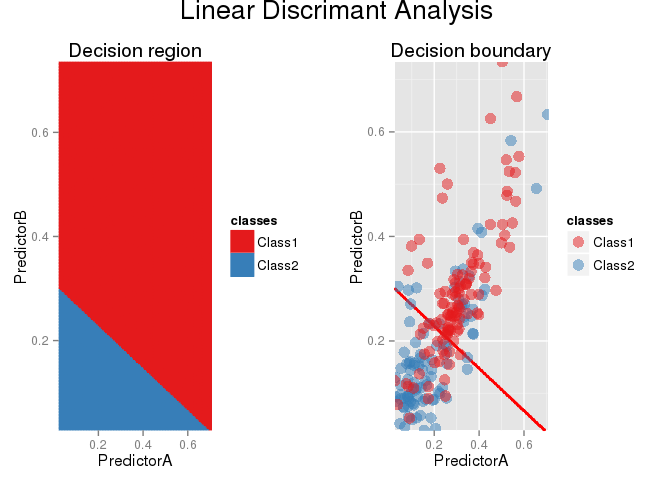
\includegraphics[height=.65\textheight]{LDA_and_QDA-1}
\end{center}
\end{frame}

\begin{frame}
\frametitle{Example: LDA }
\begin{center}
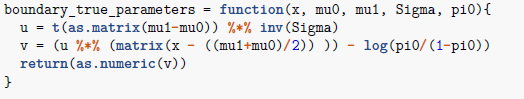
\includegraphics[width=0.8\linewidth]{./boundary_lda}
\end{center}
\begin{center}
\hspace*{-.05\textwidth}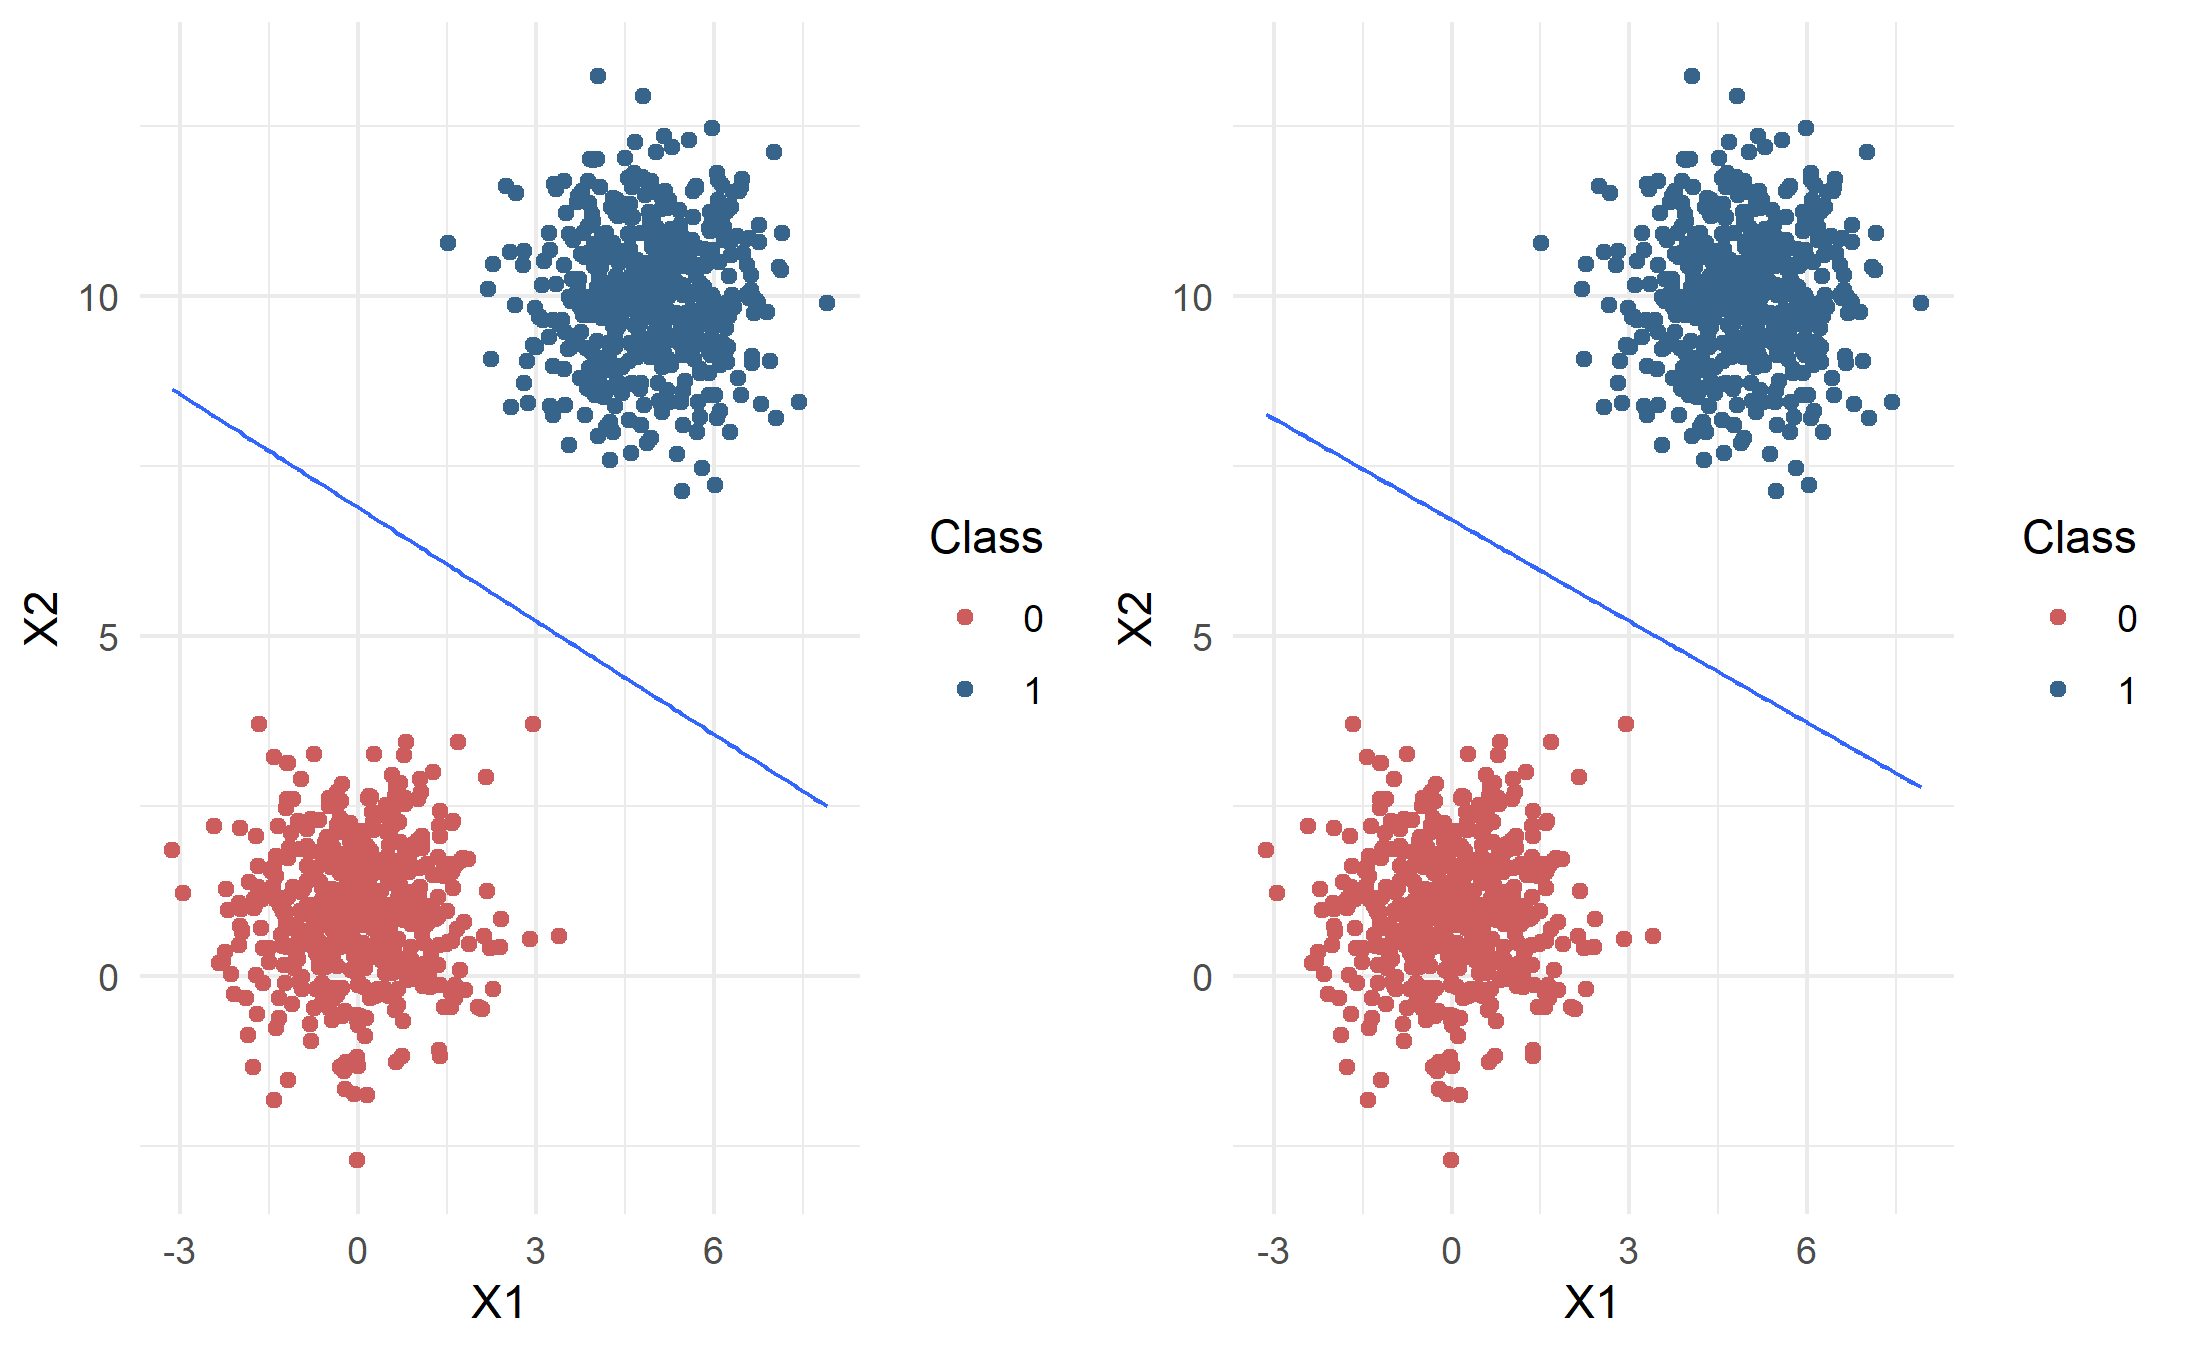
\includegraphics[height=.65\textheight]{lda_plot}
\end{center}
\end{frame}


\begin{frame}
\frametitle{Example: QDA }
\begin{center}
\hspace*{-.05\textwidth}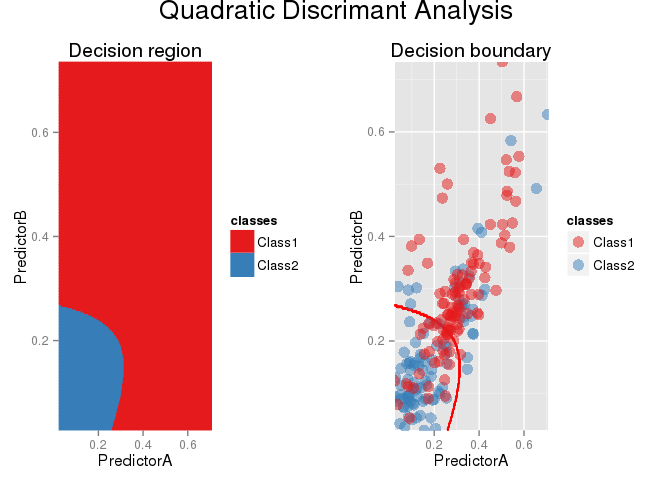
\includegraphics[height=.65\textheight]{LDA_and_QDA-2}
\end{center}
\end{frame}

\begin{frame}
\frametitle{Example: QDA }
\begin{center}
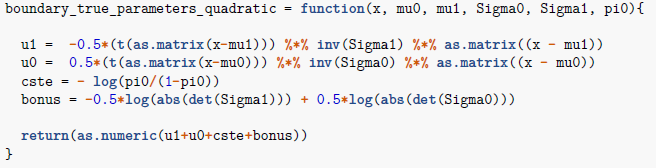
\includegraphics[width=0.8\linewidth]{./boundary_qda}
\end{center}
\begin{center}
\hspace*{-.05\textwidth}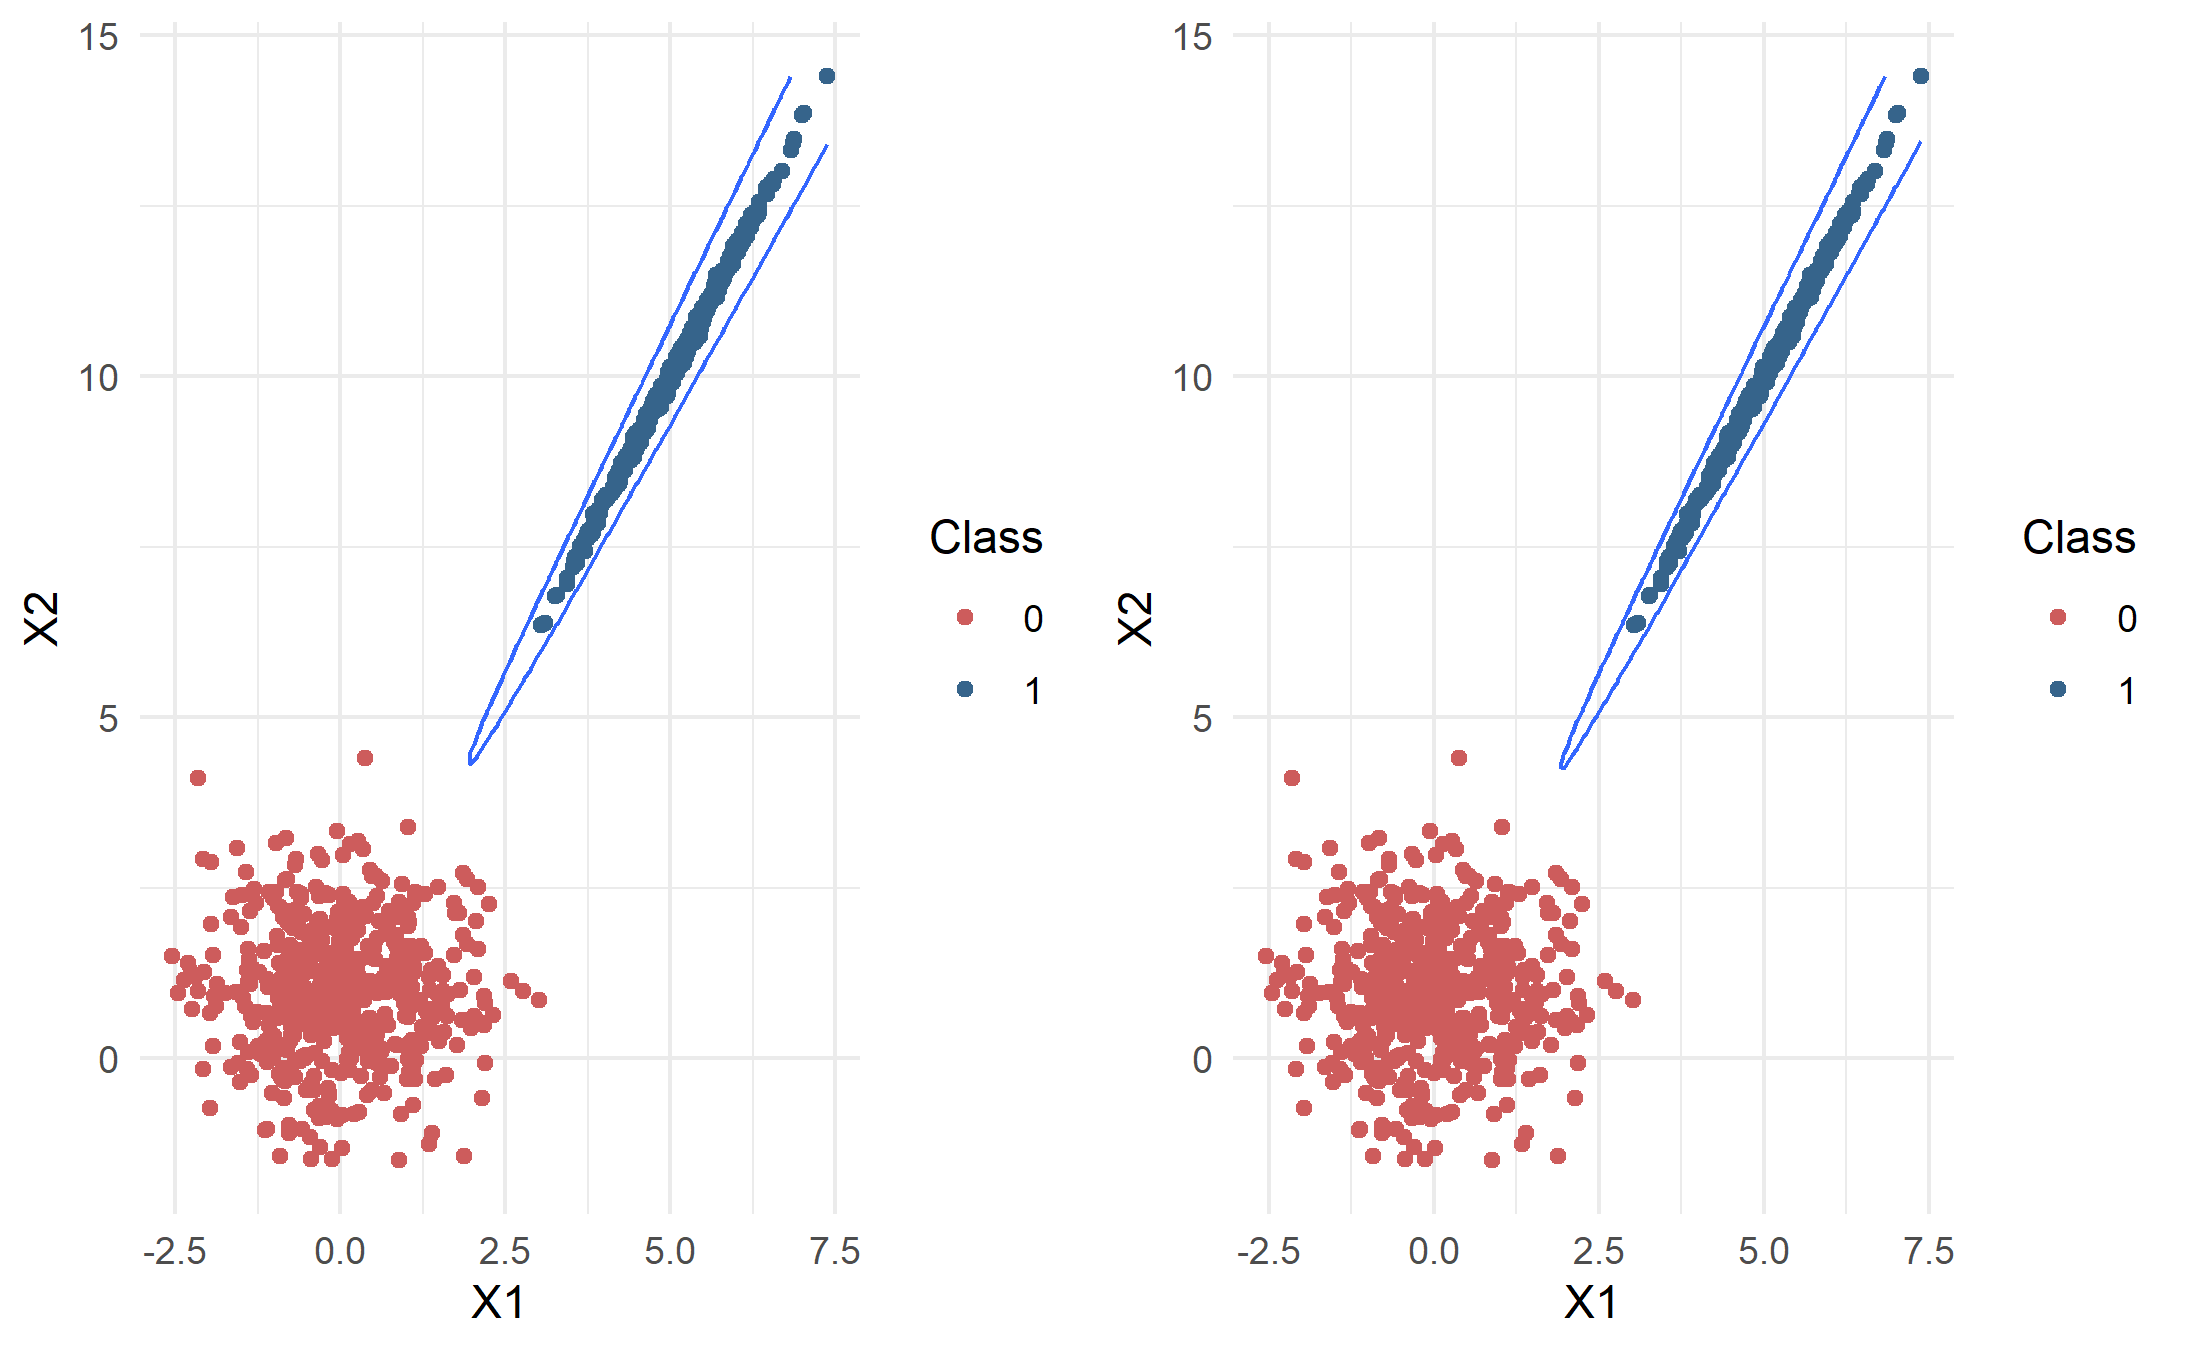
\includegraphics[height=.65\textheight]{qda_plot}
\end{center}
\end{frame}


\begin{frame}{Packages in R}

Function \textcolor{violet}{{\bf \texttt{svm}}} in package \texttt{e1071}.

\vspace{.5cm}

Function \textcolor{violet}{{\bf \texttt{lda}}} and \textcolor{violet}{{\bf \texttt{qda}}} in package \texttt{MASS}.

\vspace{.5cm}

Function \textcolor{violet}{{\bf \texttt{naive\_bayes}}} in package \texttt{naivebayes}.

\end{frame}

\section{Support Vector Machine}

\begin{frame}[t]
\frametitle{Linear classification}


$\rightharpoondown$ \alert{Simple to interpret and to implement}.

$\rightharpoondown$ On very large datasets ($n \geqslant 10^6$), no other choice (training complexity).


\medskip

\begin{center}
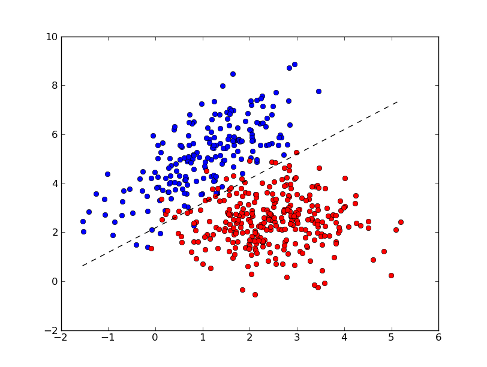
\includegraphics[width=5cm]{./lda_binary.png}
\end{center}

$\rightharpoondown$ Learn $\hat{\textbf{w}} \in \R^d$ and $\hat b$ to build the classifier:
    
\begin{align*}
\Acolorboxed{&
\hat Y = \sign(\inr{\bX, \hat{\textbf{w}}} + \hat b)\eqsp.}
\end{align*}


\end{frame}




\begin{frame}{Linearly separable data}

A dataset is \textcolor{violet}{\textbf{linearly separable}} if \alert{there exists an hyperplane $H$} (linear classification rule) such that the following assumptions hold.

$\rightharpoondown$ Points $\bX_i \in \R^d$ such that\alert{ $Y_i = 1$ are on one side of the hyperplane}.

$\rightharpoondown$ Points $\bX_i \in \R^d$ such that \alert{$Y_i = -1$ are on the other side}.

$\rightharpoondown$ $H$ \alert{does not pass through any point $\bX_i$}.


\begin{center}
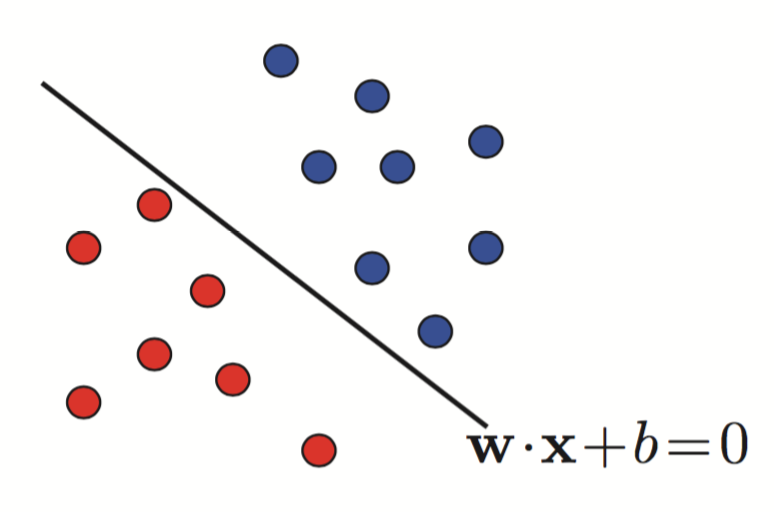
\includegraphics[width=0.75\textwidth]{./hyperplane.png}
\end{center}

\end{frame}


\begin{frame}{Some geometry}
A \textcolor{violet}{{\bf hyperplane}} is a translation of a set of vectors orthogonal to $\bw$.

\begin{align*}
\Acolorboxed{&
H_{{\bf w},b}= \{ \bx \in \R^d : \inr{\textbf{w}, \bx} + b = 0 \}\eqsp.}
\end{align*}

\vspace{.2cm}

$\rightharpoondown$ $\bw \in \R^d$ is a \textcolor{violet}{{\bf non-zero vector normal}} to the hyperplane.
$\rightharpoondown$ $b \in \R$ is a scalar. 

\vspace{.5cm}

Following for instance the results obtained for linear discriminant analysis and logistic regression, a \alert{ hyperplane $H_{\bw,b}$ may be used as a classifier} by defining

\vspace{.2cm}

\[
h_{\bw,b}: \bx \mapsto \left\{
    \begin{array}{ll}
       1 & \mbox{if }\;  \langle \bw\eqsp;\eqsp \bx\rangle + b >0\eqsp, \\
        -1 & \mbox{otherwise}\eqsp.
    \end{array}
\right.
\]
\end{frame}



\begin{frame}
\frametitle{Some geometry}

Definition of $H_{{\bf w},b}$ \alert{is invariant by multiplication of $\bw$ and $b$ by a non-zero scalar}.

\medskip

If $H_{{\bf w},b}$ does not pass through any sample point $\bx_i$,  $\bw$ and $b$ can be scaled so that

\begin{align*}
\Acolorboxed{&
\min_{(\bx, y) \in \mathcal{D}_n} |\inr{\bw, \bx} + b| = 1\eqsp.}
\end{align*}

\vspace{.2cm}

\begin{center}
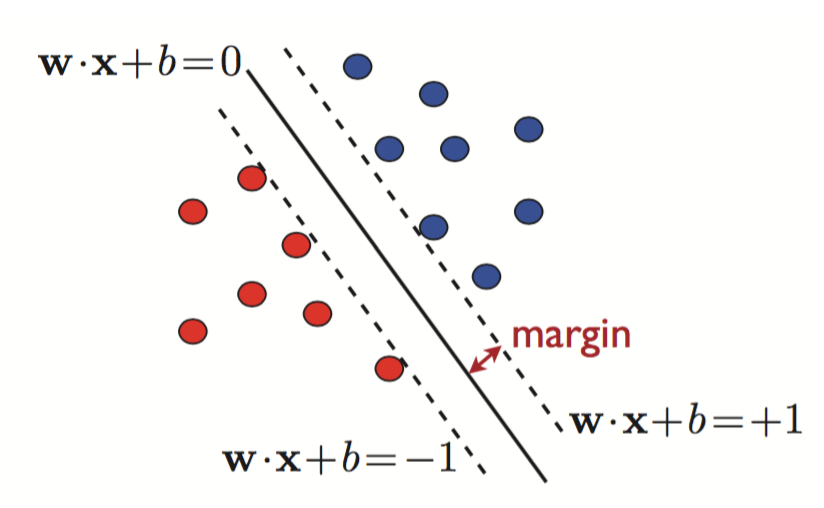
\includegraphics[width=0.5\textwidth]{canonical_hyperplane.png}
\end{center}

For such $\bw$ and $b$, we call $H$ the \alert{\emph{canonical} hyperplane}.
\end{frame}


\begin{frame}[t]
\frametitle{Some geometry}

The \alert{distance of any point $\bx' \in \R^d$ to $H_{{\bf w},b}$} is
\begin{equation*}
\frac{|\inr{\bw, \bx'} + b|}{\norm{\bw}}
\end{equation*}

If $H_{{\bf w},b}$ is a canonical hyperplane, its \alert{margin} is given by

\begin{align*}
\Acolorboxed{&
\min_{(\bx, y) \in \mathcal{D}_n}   \frac{|\inr{\bw, \bx} + b|}{\norm{\bw}} 
= \frac{1}{\norm{\bw}}\eqsp.}
\end{align*}

\begin{center}
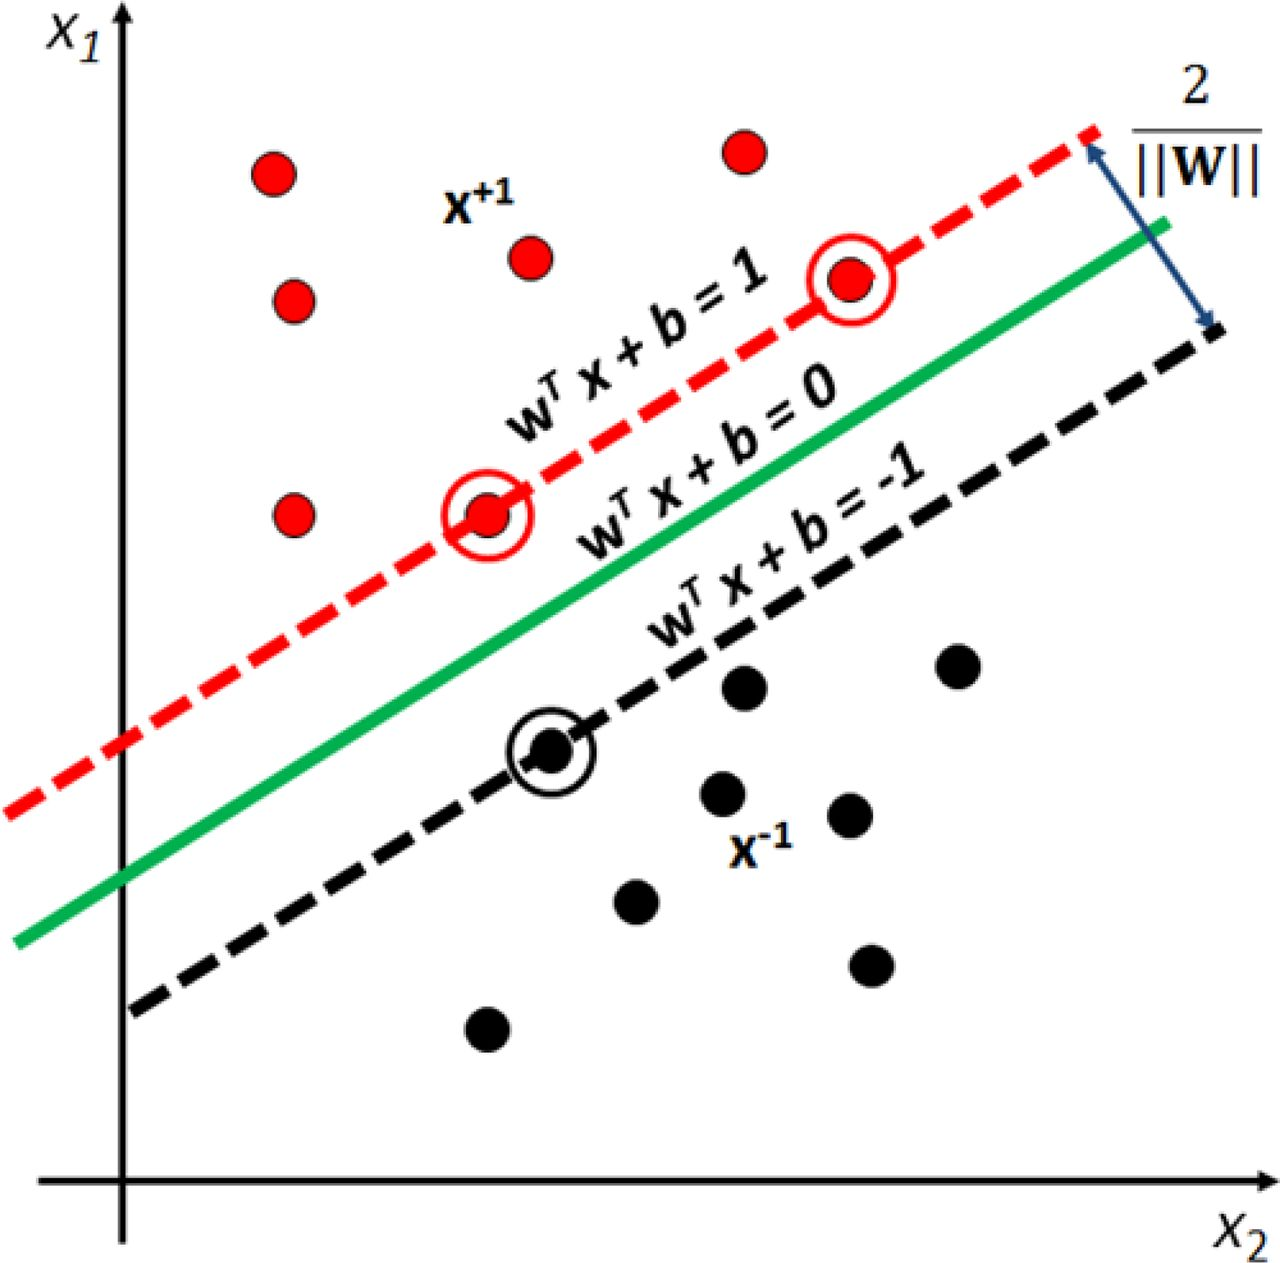
\includegraphics[width=4cm]{./margin.jpg}
\end{center}

\end{frame}


\begin{frame}
\frametitle{Linear separability and margin}

\vspace{0.2cm}
If $\mathcal{D}_n$ is \alert{strictly linearly separable}, there exists a canonical separating hyperplane 

\begin{align*}
\Acolorboxed{&
H_{{\bf w},b} = \{ \bx \in \R^d : \inr{\bw, \bx} + b = 0 \}}
\end{align*}

\vspace{.2cm}

that satisfies
\begin{equation*}
|\inr{\bw, \bX_i} + b| \geqslant 1 \; \text{ for any } \; i=1, \ldots, n\eqsp.
\end{equation*}

\vspace{0.1cm}

An individual $\bX_i$ is \alert{correctly classified} if

\vspace{0.1cm}
\begin{equation*}
Y_i (\inr{\bX_i, \bw} + b) \geqslant 1\eqsp.
\end{equation*}
\vspace{0.2cm}

The \alert{margin of $H_{{\bf w},b}$} is equal to $1 / \norm{\bw}$.
\end{frame}

\begin{frame}{Linear SVM: separable case}

\textcolor{violet}{{\bf  Hard Support Vector Machines}}  is a classification procedure which aims at  building a linear classifier with the largest possible margin, i.e. \alert{the largest minimal distance between a point in the training set and the hyperplane}.

\vspace{.5cm}

The hyperplane which \textcolor{violet}{{\bf correctly separates all training data sets with the largest margin}} is obtained with:

\vspace{.3cm}
\[
(\widehat w_n,\widehat b_n)\in \underset{\substack{(w,b)\in\mathbb{R}^d\times \mathbb{R}^d\eqsp;\eqsp \|w\|=1,\\ \forall i\in\{1,\ldots,n\},\eqsp Y_i\left(\langle w\eqsp;\eqsp \bX_i\rangle + b\right) > 0}}{\argmax}\left\{\underset{1\leqslant i \leqslant n}{\min}\;\left|\langle w\eqsp;\eqsp \bX_i\rangle + b\right|\right\}\eqsp.
\]
\end{frame}

\begin{frame}{Linear SVM: separable case}

The \textcolor{violet}{{\bf hard Support Vector Machines}} procedure is equivalent to solving the following optimization problem:

\vspace{.3cm}
\[
(\widehat w_n,\widehat b_n)\in \underset{(w,b)\in\mathbb{R}^d\times \mathbb{R}\eqsp;\eqsp \|w\|=1}{\argmax}\left\{\underset{1\leqslant i \leqslant n}{\min}\;Y_i\left(\langle w\eqsp;\eqsp X_i\rangle + b\right)\right\}\eqsp,
\]

\vspace{.5cm}

A \alert{solution to the hard Support Vector Machines optimization} problem is obtained by setting  $(\widehat w_n,\widehat b_n) = (w_\star/\|w_\star\|,b_\star/\|w_\star\|)$ where

\vspace{.3cm}

\begin{equation*}
(w_\star,b_\star)\in  \hspace{-.8cm}  \underset{\substack{(w,b)\in\mathbb{R}^d\times \mathbb{R}\\ \forall i\in\{1,\ldots,n\},\eqsp Y_i\left(\langle w\eqsp;\eqsp X_i\rangle + b\right)\geqslant 1}}{\argmin} \hspace{-.8cm} \|w\|^2\eqsp.
\end{equation*}

\end{frame}


\begin{frame}
\frametitle{Linear SVM: separable case}

A way of classifying $\mathcal{D}_n$ with maximum margin is to solve the following problem:

\vspace{.2cm}

\begin{align*}
\Acolorboxed{&
(w_\star,b_\star)\in  \hspace{-.8cm}  \underset{\substack{(w,b)\in\mathbb{R}^d\times \mathbb{R}\\ \forall i\in\{1,\ldots,n\},\eqsp Y_i\left(\langle w\eqsp;\eqsp X_i\rangle + b\right)\geqslant 1}}{\argmin} \hspace{-.8cm} \|w\|^2\eqsp.}
\end{align*}

\vspace{.2cm}

$\rightharpoondown$ This problem \alert{admits a \textbf{unique} solution}.
 
$\rightharpoondown$ It is a \textcolor{violet}{{\bf quadratic programming}} problem, which is easy to solve numerically.

$\rightharpoondown$ Dedicated optimization algorithms can \alert{solve this on a large scale very efficiently}.

\end{frame}


\begin{frame}[t]
\frametitle{Linear SVM: separable case}

The optimization problem is solved using \alert{Karush-Kuhn-Tucker's theorem}.

\medskip

There are $\alpha_i \geqslant 0$, $i=1, \ldots, n$, called \alert{dual variables}, such that the solution $(\bw, b)$ of this problem satisfies:

\vspace{.3cm}

\begin{align*}
\Acolorboxed{&\bw = \sum_{i=1}^n \alpha_i Y_i \bX_i \;\; \text{ and } \;\;
\alpha_i ((Y_i \inr{\bw, \bX_i} + b) - 1) = 0 \; \text{ for } \; i=1, \ldots, n\eqsp.}
\end{align*}

\vspace{.2cm}

$\rightharpoondown$ $\alpha_i \neq 0$ if and only if $Y_i \inr{\bw, \bX_i} + b = 1$, meaning that \alert{$\bX_i$ is on the marginal hyperplane}.


$\rightharpoondown$ Weights vector $\bw$ is a \alert{linear combination of the vectors $\bx_i$} that belong to a marginal hyperplane.


$\rightharpoondown$ Such points $\bx_i$ are called \textcolor{violet}{{\bf support vectors}}.
\end{frame}


\begin{frame}
\begin{center}
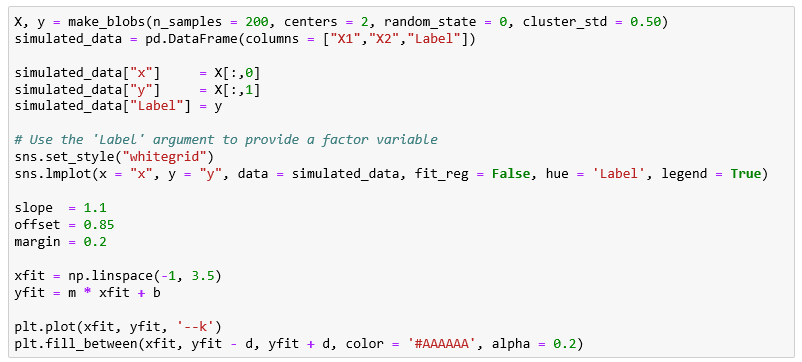
\includegraphics[width=0.8\textwidth]{svm_data1.png}
\end{center}
\end{frame}

\begin{frame}
\begin{center}
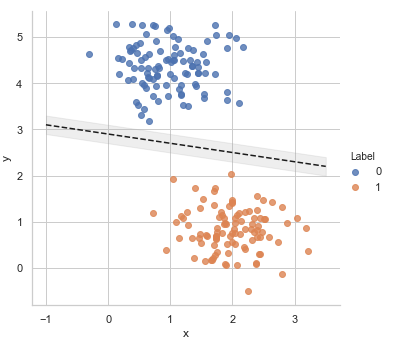
\includegraphics[width=0.8\textwidth]{svm_data2.png}
\end{center}
\end{frame}

\begin{frame}
\begin{center}
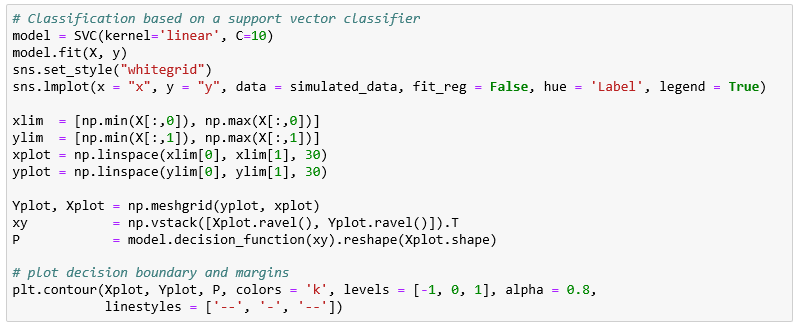
\includegraphics[width=0.8\textwidth]{svm_linear1.png}
\end{center}
\end{frame}

\begin{frame}
\begin{center}
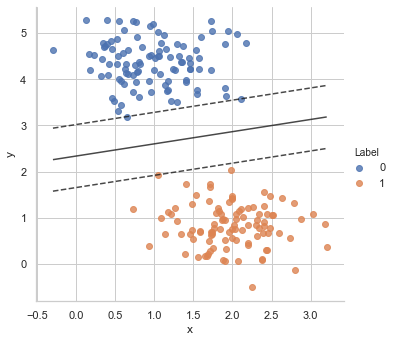
\includegraphics[width=0.8\textwidth]{svm_linear2.png}
\end{center}
\end{frame}

\begin{frame}
\begin{center}
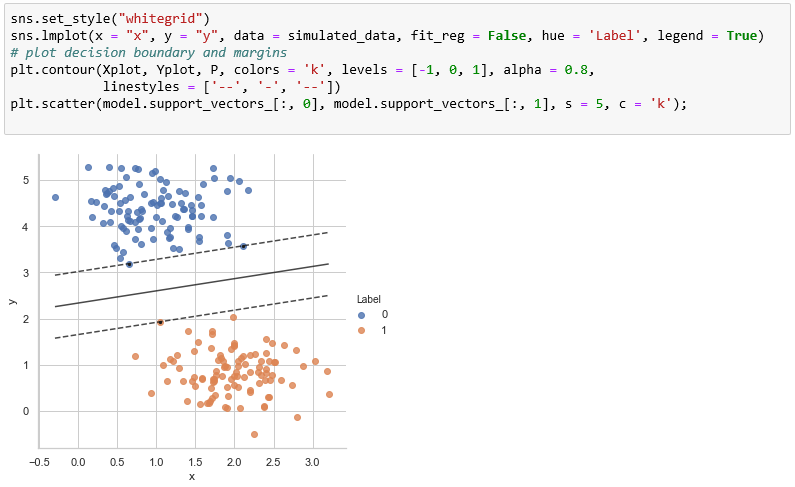
\includegraphics[width=0.8\textwidth]{svm_linear3.png}
\end{center}
\end{frame}

\begin{frame}[t]
\frametitle{Linear SVM: non-separable case}

Have you ever seen a dataset that looks that this?
\begin{center}
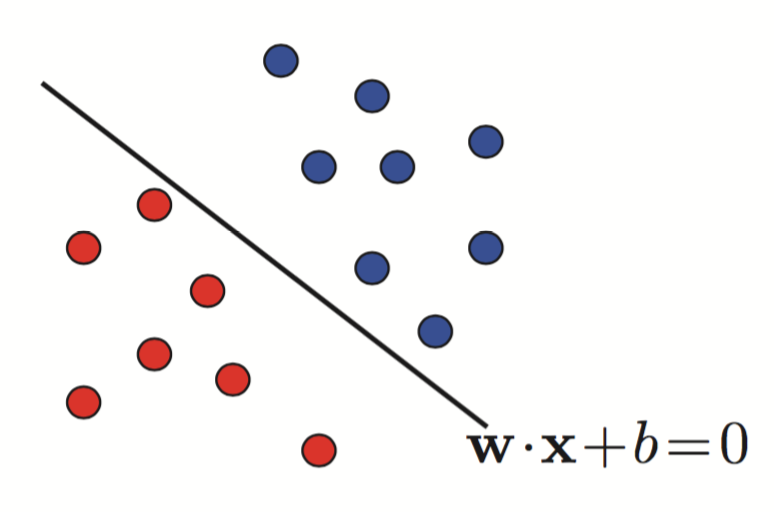
\includegraphics[width=0.4\textwidth]{hyperplane.png}
\end{center}

$\rightharpoondown$ Restricting the problem to linearly separable  training data sets is a \alert{somehow strong assumption}.

$\rightharpoondown$ Inequality constraints in the quadratic optimization problem \alert{can be relaxed}.

$\rightharpoondown$ Introduction of nonnegative variables $(\xi_i)_{1\leqslant i \leqslant n}$ which \textcolor{violet}{quantify the nonfeasability of the constraint} $Y_i(\langle \bw\eqsp;\eqsp \bX_i\rangle + b)\geqslant 1$.

\begin{equation*}
Y_i (\inr{\bw, \bX_i} + b) \geqslant 1 - \xi_i\eqsp.
\end{equation*}

\end{frame}


\begin{frame}
\frametitle{Linear SVM: non-separable case}

The original problem is then replaced by

\begin{equation*}
(w_\star,b_\star,\xi_\star)\in  \hspace{-.8cm}  \underset{\substack{(w,b,\xi)\in\mathbb{R}^d\times \mathbb{R}\times\mathbb{R}_+^d\\ \forall i\in\{1,\ldots,n\},\eqsp Y_i\left(\langle w\eqsp;\eqsp X_i\rangle + b\right)\geqslant 1-\xi_i}}{\argmin} \hspace{-.5cm} \left\{\lambda\|w\|^2 + \frac{1}{n}\sum_{i=1}^n\xi_i\right\}\eqsp,
\end{equation*}
where $\lambda >0$.

\vspace{.3cm}

The \textcolor{violet}{{\bf soft Support Vector Machines}} algorithm minimizes \alert{simultaneously the margin of the linear classifier and the average value of these slack variables}.

\vspace{.3cm}

Note that, if $(w_\star,b_\star)$ is solution to
\begin{equation*}
(w_\star,b_\star)\in  \underset{(w,b)\in\mathbb{R}^d\times \mathbb{R}}{\argmin}  \left\{\lambda\|w\|^2 + \frac{1}{n}\sum_{i=1}^n(1-Y_i\left(\langle w\eqsp;\eqsp X_i\rangle + b\right))_+\right\}\eqsp,
\end{equation*}
then $(w_\star/\|w_\star\|,b_\star,\xi_\star/\|w_\star\|)$ is solution to \alert{the soft SVM problem}.
\end{frame}



\begin{frame}
\frametitle{Linear SVM: non-separable case}

The \textcolor{violet}{{\bf soft SVM problem boils down}} to computing:
\begin{equation*}
(w_\star,b_\star,\xi_\star)\in  \hspace{-.8cm}  \underset{\substack{(w,b,\xi)\in\mathbb{R}^d\times \mathbb{R}\times\mathbb{R}_+^d\\ \forall i\in\{1,\ldots,n\},\eqsp Y_i\left(\langle w\eqsp;\eqsp X_i\rangle + b\right)\geqslant 1-\xi_i}}{\argmin} \hspace{-.5cm} \left\{\lambda\|w\|^2 + \frac{1}{n}\sum_{i=1}^n\xi_i\right\}\eqsp,
\end{equation*}
where $\lambda >0$.

\vspace{.3cm}

$\rightharpoondown$ This problem \alert{admits a \textbf{unique} solution}.
 
$\rightharpoondown$ It is a \textcolor{violet}{{\bf quadratic programming}} problem, which is easy to solve numerically.

$\rightharpoondown$ Dedicated optimization algorithms can \alert{solve this on a large scale very efficiently}.



\end{frame}



\begin{frame}{The hinge loss}

This problem can be reformulated as follows

\begin{equation*}
\argmin_{\bw \in \R^d, b \in \R} \left\{\frac 12 \norm{\bw}_2^2 + C \sum_{i=1}^n \max\Big(0, 1 - y_i (\inr{\bx_i, \bw} + b) \Big)\right\}\eqsp,
\end{equation*}

\vspace{0.2cm}

By introducing the \alert{hinge loss}

\begin{equation*}
\ell(y, y') = \max(0, 1 - y y') = (1 - y y')_+,
\end{equation*}

\vspace{0.2cm}
the problem can be written as

\begin{equation*}
\argmin_{\bw \in \R^d, b \in \R} \left\{\frac 12 \norm{\bw}_2^2 + C \sum_{i=1}^n \ell(y_i, \inr{\bx_i, \bw} + b)\right \}\eqsp.
\end{equation*}

\vspace{0.2cm}

$\rightharpoondown$ Specific  loss functions $\ell$ in a \alert{general setting}.

\end{frame}

\begin{frame}{Introduction to nonparametric classification}
The joint law of $(X,Y)$ is \textcolor{violet}{{\bf not assumed to belong to any parametric or semiparametric}} family of models. 


\vspace{.4cm}

The classification risk {\bf cannot be computed nor  minimized}, it is instead estimated by the empirical classification risk defined as
\[
\widehat L^n_{\mathrm{miss}}(f) = \frac{1}{n}\sum_{i=1}^n \mathds{1}_{Y_i \neq f(\vecX_i)}\,,
\]
where  $(X_i,Y_i)_{1\leqslant i\leqslant n}$ are independent  with the same distribution as $(X,Y)$. 

\vspace{.4cm}

The classification problem then boils down to solving
\[
\widehat f^n \in \underset{f\in\mathcal{F}}{\argmin}\;\widehat L^n_{\mathrm{miss}}(f)\eqsp,
\]
for a chosen class $\mathcal{F}$ of classifiers.
\end{frame}

\begin{frame}{Introduction to nonparametric classification}
Nonparametric classification based on the empirical risk minimization may seem appealing  

It cannot be used to derive efficient practical classifiers due to \textcolor{violet}{{\bf the computational cost of the optimization problem}}. 

The target loss function $\widehat L^n_{\mathrm{miss}}$ is replaced by \textcolor{violet}{{\bf a convex surrogate and its minimization is constrained to a convex set of classifiers}}.

\vspace{.3cm}

For any convex function $\phi:\mathcal{X}\to \mathbb{R}$, it is possible to build a classifier $f$ given by $f_\phi=\mathrm{sign}(\phi)$. The associated empirical classification is then
\[
\widehat L^n_{\mathrm{miss}}(\phi) = \frac{1}{n}\sum_{i=1}^n \mathds{1}_{Y_i \neq f_\phi(X_i)} = \frac{1}{n}\sum_{i=1}^n \mathds{1}_{Y_i\phi(X_i) <0}\,.
\]
\end{frame}

\begin{frame}{Introduction to nonparametric classification}
Replacing the indicator function by \textcolor{violet}{{\bf any convex loss funtion $\ell$ yields a convex surrogate}}:
\[
\widehat L^{n,\mathrm{conv}}_{\mathrm{miss}}(\phi) = \frac{1}{n}\sum_{i=1}^n \ell(Y_i\phi(X_i))\eqsp.
\]

\vspace{.3cm}

Penalizing the smoothness of the function $\phi$ is penalized, $\widehat L^{n,\mathrm{conv}}_{\mathrm{miss}}$ may be  replaced by 
\[
\widehat L^{n,\mathrm{conv}}_{\mathrm{miss}}(\phi) = \frac{1}{n}\sum_{i=1}^n \ell(Y_i\phi(X_i)) + \lambda\|\phi\|^2\,,
\]
where $\lambda>0$ and $\|\cdot\|$ is a norm on the space $\mathcal{H}$. 

\vspace{.3cm}

\textcolor{violet}{{\bf The soft Support Vector Machines}} algorithm fits this framework with the affine base function $\phi:\bx\mapsto \langle \bw\eqsp;\eqsp \bx\rangle + b$ and $\ell$ chosen as the hinge loss $\ell: x \mapsto (1-x)_+$ when the target function is penalized by its margin $\|w\|^2$.

\end{frame}

\begin{frame}{Kernel trick}
A useful case in practice consists in choosing $\mathcal{H}$ as a \textcolor{violet}{{\bf Reproducing Kernel Hilbert Space}} with positive definite kernel $k$ on $\mathcal{X}\times \mathcal{X}$.

\vspace{.3cm}

A function $k$ on $\mathcal{X}\times \mathcal{X}$ is said to be \textcolor{violet}{{\bf a positive definite kernel}} if and only if it is symmetric and if for all $n\geqslant 1$, $(x_1,\ldots,x_n)\in\mathcal{X}^n$ and all $(a_1,\ldots,a_n)\in\mathbb{R}^n$,

\vspace{.15cm}

\[
\sum_{1\leqslant i,j\leqslant n}a_ia_jk(x_i,x_j) \geqslant 0\,.
\]

\vspace{.3cm}

The \textcolor{violet}{{\bf Reproducing Kernel Hilbert Space}} with kernel $k$ is the only Hilbert space $\mathcal{H} \subset \mathbb{R}^\mathcal{X}$ such that for all $x\in\mathcal{X}$,  $k(x,\cdot) \in \mathcal{H}$ and for all $x\in\mathcal{X}$ and all $f\in\mathcal{H}$,
\[
f(x) = \langle f\,;\, k(x,\cdot)\rangle_\mathcal{H}\,.
\]

\end{frame}

\begin{frame}{Kernel trick}
$k:\mathcal{X}\times\mathcal{X}:\to \mathbb{R}$ a positive definite kernel and $\mathcal{H}$ the RKHS with kernel $k$. 

\vspace{.1cm}
 
\[
\textcolor{lightr}{\widehat \phi^n_{\mathcal{H}} \in \underset{\phi\in\mathcal{H}}{\argmin}\;\frac{1}{n}\sum_{i=1}^n \ell(Y_i\phi(X_i)) + \lambda\|\phi\|_\mathcal{H}^2\,,}
\]

\vspace{.1cm}

where $\|\phi\|^2_\mathcal{H} = \langle \phi\eqsp;\eqsp \phi\rangle$, is given by 

\vspace{.1cm}

\[
\widehat \phi^n_{\mathcal{H}} : x \mapsto \sum_{i=1}^n \widehat \alpha_i k(X_i,x)\,,
\]
with

\vspace{.1cm}

\[
\textcolor{violet}{\widehat\alpha \in \underset{\alpha \in \mathbb{R}^n}{\argmin}\;\left\{\frac{1}{n}\sum_{i=1}^n \ell\left(\sum_{j=1}^n\alpha_jY_ik(X_j,X_i)\right) + \lambda \sum_{1\leqslant i,j \leqslant n}\alpha_i \alpha_j k(X_i,X_j)\right\}\,.}
\]
\end{frame}
%
%\begin{frame}{The hinge loss}
%Another natural loss is the $0/1$ loss given by
%\begin{equation*}
%\ell_{0/1}(y, z) = \ind{yz \leq 0}.
%\end{equation*}  
%Instead of the Linear SVM, it would be nice to consider
%\begin{equation*}
%\argmin_{w \in \R^d, b \in \R} \frac 12 \norm{w}_2^2 + C \sum_{i=1}^n 
%\ind{y_i (\inr{x_i, w} + b) \leq 0},
%\end{equation*}
%but impossible numerically (NP-hard)
%
%\begin{tabular}[htbp]{cc}    
%\begin{minipage}[htbp]{.5\linewidth}
%Hinge loss is as a \textbf{convex surrogate} 
%for the $0/1$ loss
%\end{minipage}
%&
%\begin{minipage}[htbp]{.5\linewidth}
%\vspace{0.2cm}
%\begin{center}
%\includegraphics[width=5cm]{hinge_loss.png}
%\end{center}
%\end{minipage}
%\end{tabular}
%\end{frame}
%
%
%\begin{frame}
%\frametitle{What we've seen so far}
%
%\textbf{Linear classification problem}
%\begin{tabular}[htbp]{cc}    
%\begin{minipage}[htbp]{.5\linewidth}
%\vspace{0.2cm}
%\begin{center}
%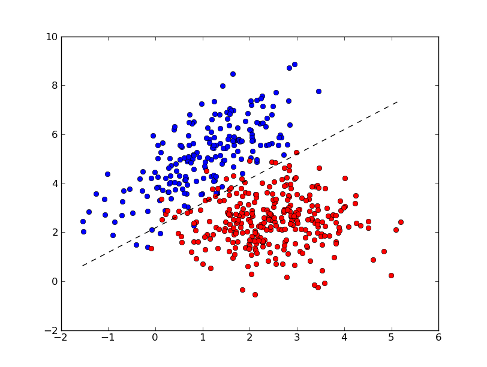
\includegraphics[width=4cm]{lda_binary.png}
%\end{center}
%\end{minipage}
%&
%\begin{minipage}[htbp]{.5\linewidth}
%Learn $\hat w \in \R^d$ and $\hat b$ such that       
%\begin{equation*}
%\hat y = \sign(\inr{x, \hat w} + \hat b)
%\end{equation*}
%is a good classifier
%\end{minipage}
%\end{tabular}
%
%\bigskip
%
%\textbf{A solution: linear SVM}
%
%Find $\hat w \in \R^d$ and $\hat b \in \R$ given by
%\begin{equation*}
%(\hat w, \hat b) = \argmin_{w \in \R^d, b \in \R} \frac 12 \norm{w}_2^2 
%+ C \sum_{i=1}^n \ell(y_i, \inr{x_i, w} + b)
%\end{equation*}
%where $\ell(y, y') = (1 - y y')_+$ is the \textbf{hinge} loss.
%\end{frame}





\end{document}
%%% Local Variables: 
%%% mode: latex
%%% TeX-master: t
%%% End: 
